
\section{統計的仮説検定}
ここまで、推測ができるまたは、データが統計モデルにおいてよくある値なのかを利用し、統計モデルの良さを評価し、良いモデルを選択しようとした。
統計的仮説検定では、絶対にダメな統計モデルを調べる方法である。
\begin{defi}
    データと統計モデルを比較して、絶対にだめと判断されたとき、統計モデルを棄却すると宣言する。絶対にダメと判断されないときは、統計モデルを採択(棄却の対義語)するとは宣言しない。統計モデルが棄却されるのは、統計モデルの仮定によって変化する。本書の範囲内であれば、統計モデルの母数、分布関数、独立同一の分布関数からサンプリングされたことによる。特に、統計モデルの母数の変化によって決まる棄却される母数の範囲を棄却域といい、棄却されない母数の範囲を信頼区間という。サンプルから得られる統計量以上の値が得られる確率を$p$値と呼ぶ。棄却される$p$値の閾値を有意水準$\alpha$と言い、一般に$\alpha=0.05$が使われる。統計モデルの分布関数が変化すれば、その統計モデルにおける信頼区間・棄却域・$p$値の計算方法も変わる。
\end{defi}

\if 0 
これらの事象は、統計モデルの上で観測される、数学的な事実です。
数学を扱っている以上はこの事実は決して崩れることはありえません。
一方で、我々が扱う現象ではどうなるでしょうか。現象が数学な分布関数から生成されていることは決してありえません。
誰かがサイコロを振って、人々の身長を決めているのなら話は別ですが、
人の身長が、ランダムに正規分布によって決定されることはありませんね。

$M(168)$モデルの平均値は$168cm$、データでは$171cm$程度なので、$3cm$小さい。また、
$180cm$以上の人の割合を使ってモデルとデータの乖離を調べることができました。
$180cm$の人がたまたまいなかった場合は、$M(169.1),M(168)$のどちらも推測できているとは言い難いことになります。このことから、特定の値を使って乖離を判定することは難しいと考えられます。


$\phi(z>Z(\mu))を$p値として、絶対に選択してはいけない統計モデル$M(\mu)$の母数$\mu$を調べます。具体的には、指標$p$が$0.05$より小さい統計モデルを選択しないようにします。その母数の範囲は$162.14 >\mu, \mu > 174.31$です。この母数の統計モデルは$p=0.05$の基準で使わないことを統計モデルを棄却すると言います。逆に、$p>0.05$となるモデルは、積極的に正しいとは考えません。明らかに間違いではないけども正しくもないという判断をします。


$p$値を使う方法がとられます。p値とは統計モデルとデータの乖離度合いを示す指標です。p値は$0~1$の値をとり、$0$に近いと統計モデルとデータが乖離していると判断します。
\fi 

これまでは、統計モデル$M(\mu)$における信頼区間・棄却域の計算を行ってきました。今回は、$p$値を計算します。
無作為抽出により得られたデータ$\bar{x}$がこれ以上偏る確率は、
$\phi(z>\frac{\sqrt{n}(\bar{x}-\mu)}{\sigma})$
により計算できます。

図1は、$\mu$を変数にし、各$\mu$に対して、$\phi(z>Z(\mu))$を示します。標本平均$168.7cm$をピークに左右対象に$\phi(z>Z(\mu))$が減少していることが分かります。つまり、$M(168.7)$が最も乖離の度合いが小さい統計モデルです。
\begin{figure}
\begin{center}
   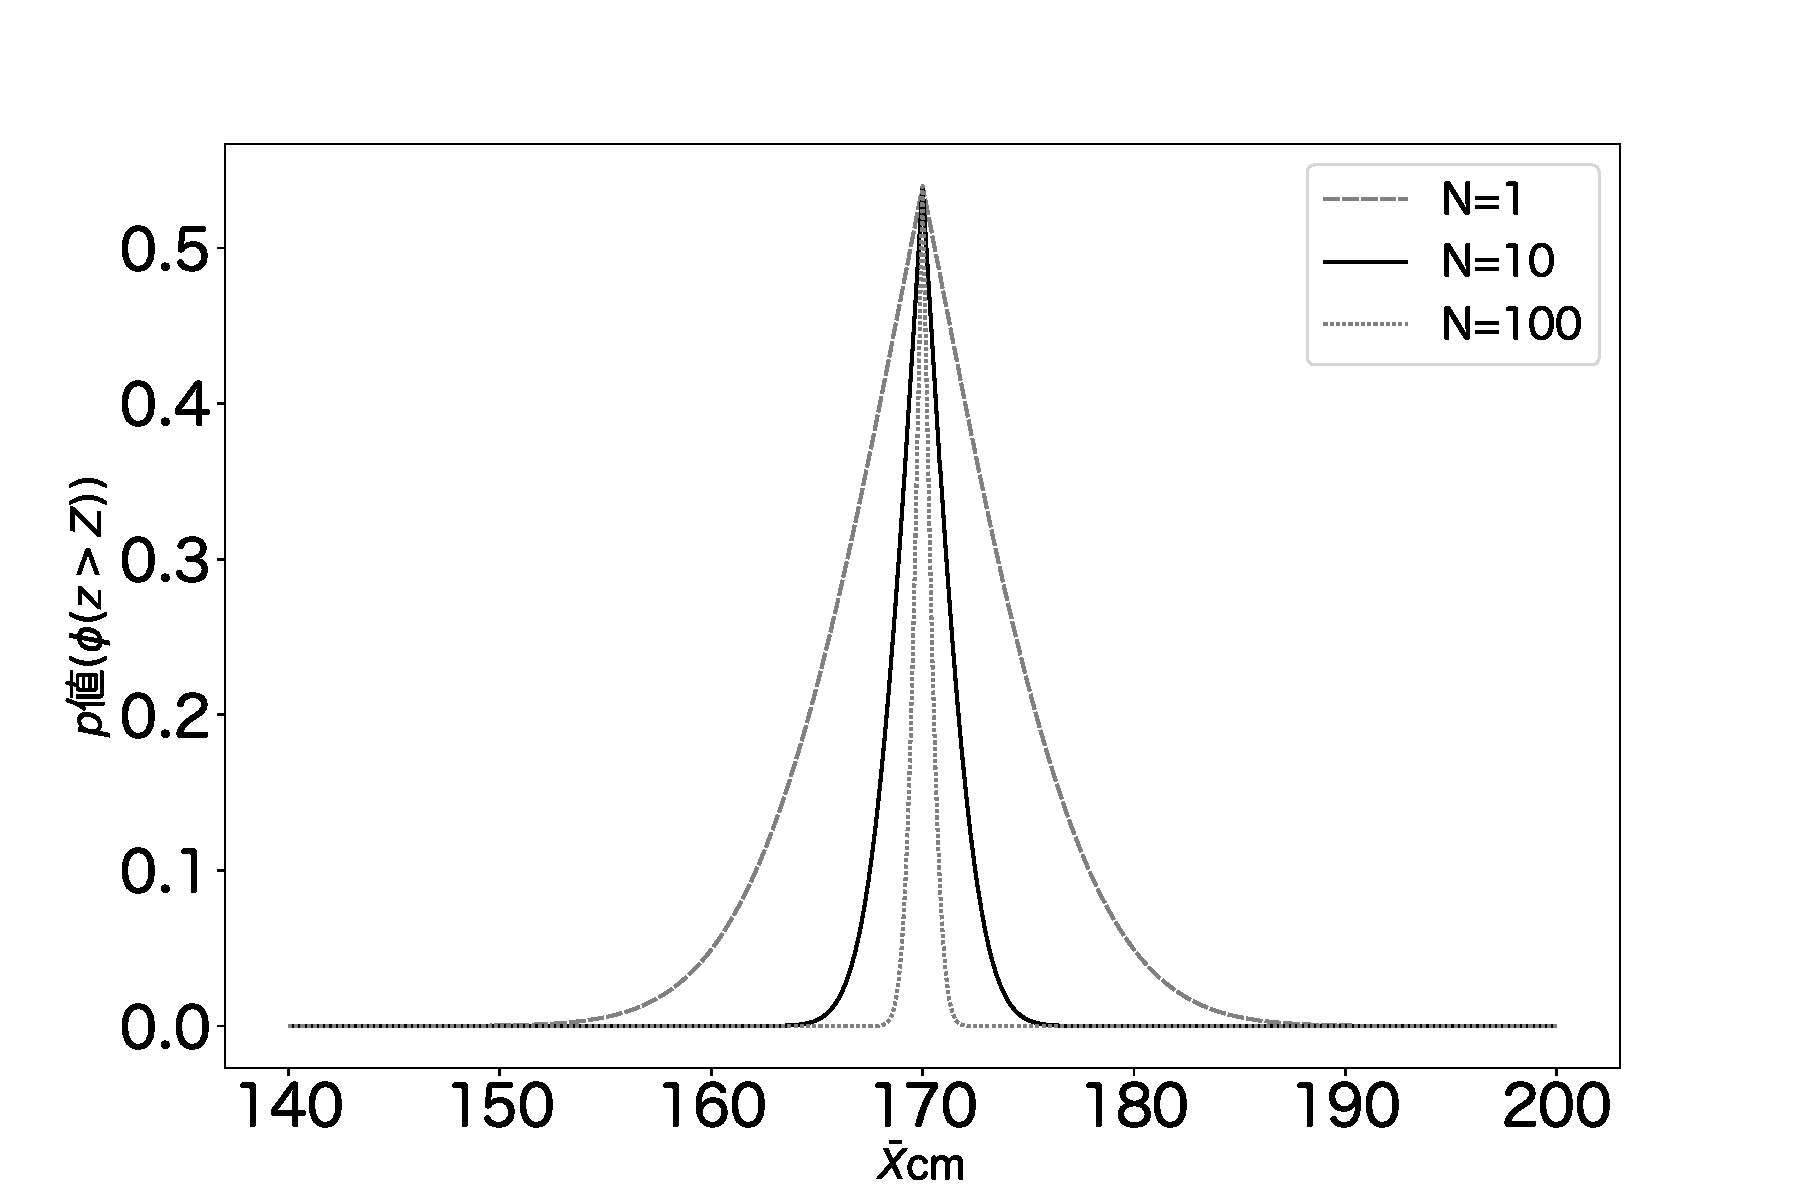
\includegraphics[width=15cm]{./image/04_/p_cm.pdf}
   %\caption{図1.p値cm}
 \end{center}
\end{figure}



 \if 0 

このとき、$Z(\bar{x},\mu)$が$N(0,1)$においてよくある値でない場合に、棄却します。
一方で、$Z(\bar{x},\mu)$が$N(0,1)$においてよくある値だったとしても、統計モデルを採用するとは言いません。
また、$Z(\bar,\mu)$の絶対値が$0$よりも十分大きな値を取れば、$N(0,1)$において出にくいということがわかります。これは、$|\bar{X}-\mu|$つまり、統計モデルの母数$\mu$と平均値$\bar{X}$の絶対値が大きければ、$Z(\bar{X},\mu)$の出現頻度は低く、絶対値が十分$0$に近ければ、$Z(\bar{X},\mu)$の出現頻度は高いことを意味します。

ここまでは、全て数学的フィクションである統計モデルの話をしました。では、現実のデータが
では、p値が語っていることを考えるいきます。


以上のことから、この検定を使うには、少なくともQ-Qプロットが必要であることが分かります。


一般に、統計モデルが棄却されない母数の領域を信頼区間といい、棄却される母数の領域を棄却区間という。
特に、$p=0.05$を基準とし、その基準における統計モデルが棄却されない区間を$95\%$ ($100*(1-0.05)$)信頼区間という。


信頼区間と対応する言葉として、採択域(棄却域)というものがある。棄却域は、確率変数を標準正規分布へ変数変換した後での信頼区間である。これは明らかに信頼区間と一対一対応する。

https://twitter.com/genkuroki/status/1270179975195316224


信頼区間は、データによって棄却されない母数の範囲のことである。

信頼区間は、統計モデルが棄却されるパラメータかどうかを表しているので、現実の推論を全く行っていない。

身長を統計モデルにより扱うことで、$p<0.05$では帰無仮説が棄却され、推測を行う統計モデルとはいまいちだということは分かったと思う。一方で、$p>0.05$となった場合でも積極的に採択しないことはなぜだろうか。次は、その理由を探る。
\fi
\subsubsection{統計モデルを積極的に採用しない理由}
設定した$\alpha=0.05$よりも大きな$p$値をもつ統計モデル$M(162.2)$は、それなりに推測するでしょうか。この統計モデルにより$P(x=170)$は、極めて少数であり、サンプルサイズを大きくしたときと乖離していることが分かります。このことから、全ての現象に対して特定の$p$値を元に棄却するモデルを決めることの無意味さを感じることができます。

p値が小さいとき、統計モデルの少なくとも一つの仮定と実際のデータとが合わないことが考えられます。そこでまず、統計モデルの仮定を満たしているのかを確認します。統計モデルの仮定(1)を確認します。身長データを無作為抽出して計測したため、身長データはそれぞれ独立であると考えられます。次に統計モデルの仮定(2)です。これは、Q-Qプロットを使います。もし、データが正規分布ではなさそうであれば、この統計モデルは使えません。
以上のことが確かめられたら統計モデルの仮定(3)が実際のデータと異なると結論付けます。少なくとも、ある母数では実際のデータと乖離していると主張するわけです。



実際に、検定を行なっておく。$N=1,\bar{x}=181$とする。このとき、$\bar{x}\sim N(\mu,\sigma^2)$より、$\frac{\sqrt{n}(170-\bar{x})}{\sigma}=-1.61$より、$z_{0.975}=-2.241$なので、棄却域に含まれない。統計モデル$M(170)$は棄却されない。
$N=4,\bar{x}=181$とする。このとき、$\frac{\sqrt{n}(170-\bar{x})}{\sigma}=-3.23$より、棄却されることがわかる。

棄却されるモデルが観測されたデータの平均値$\bar{x}$に応じて変化することを視覚的に確認しておく。図はさまざまな$\bar{x}$を得たときにその信頼区間を描いたものである。この信頼区間の範囲内にある$\mu$であれば、統計モデル$M(\mu)$は棄却されない。例えば、$\bar{x}=170$であれば、$M(170)$は棄却されない。一方で、$\bar{x}=165$あたりであれば、その棄却域は$\mu=170$を含まないので、$M(170)$は棄却される。

\begin{figure}
\begin{center}
    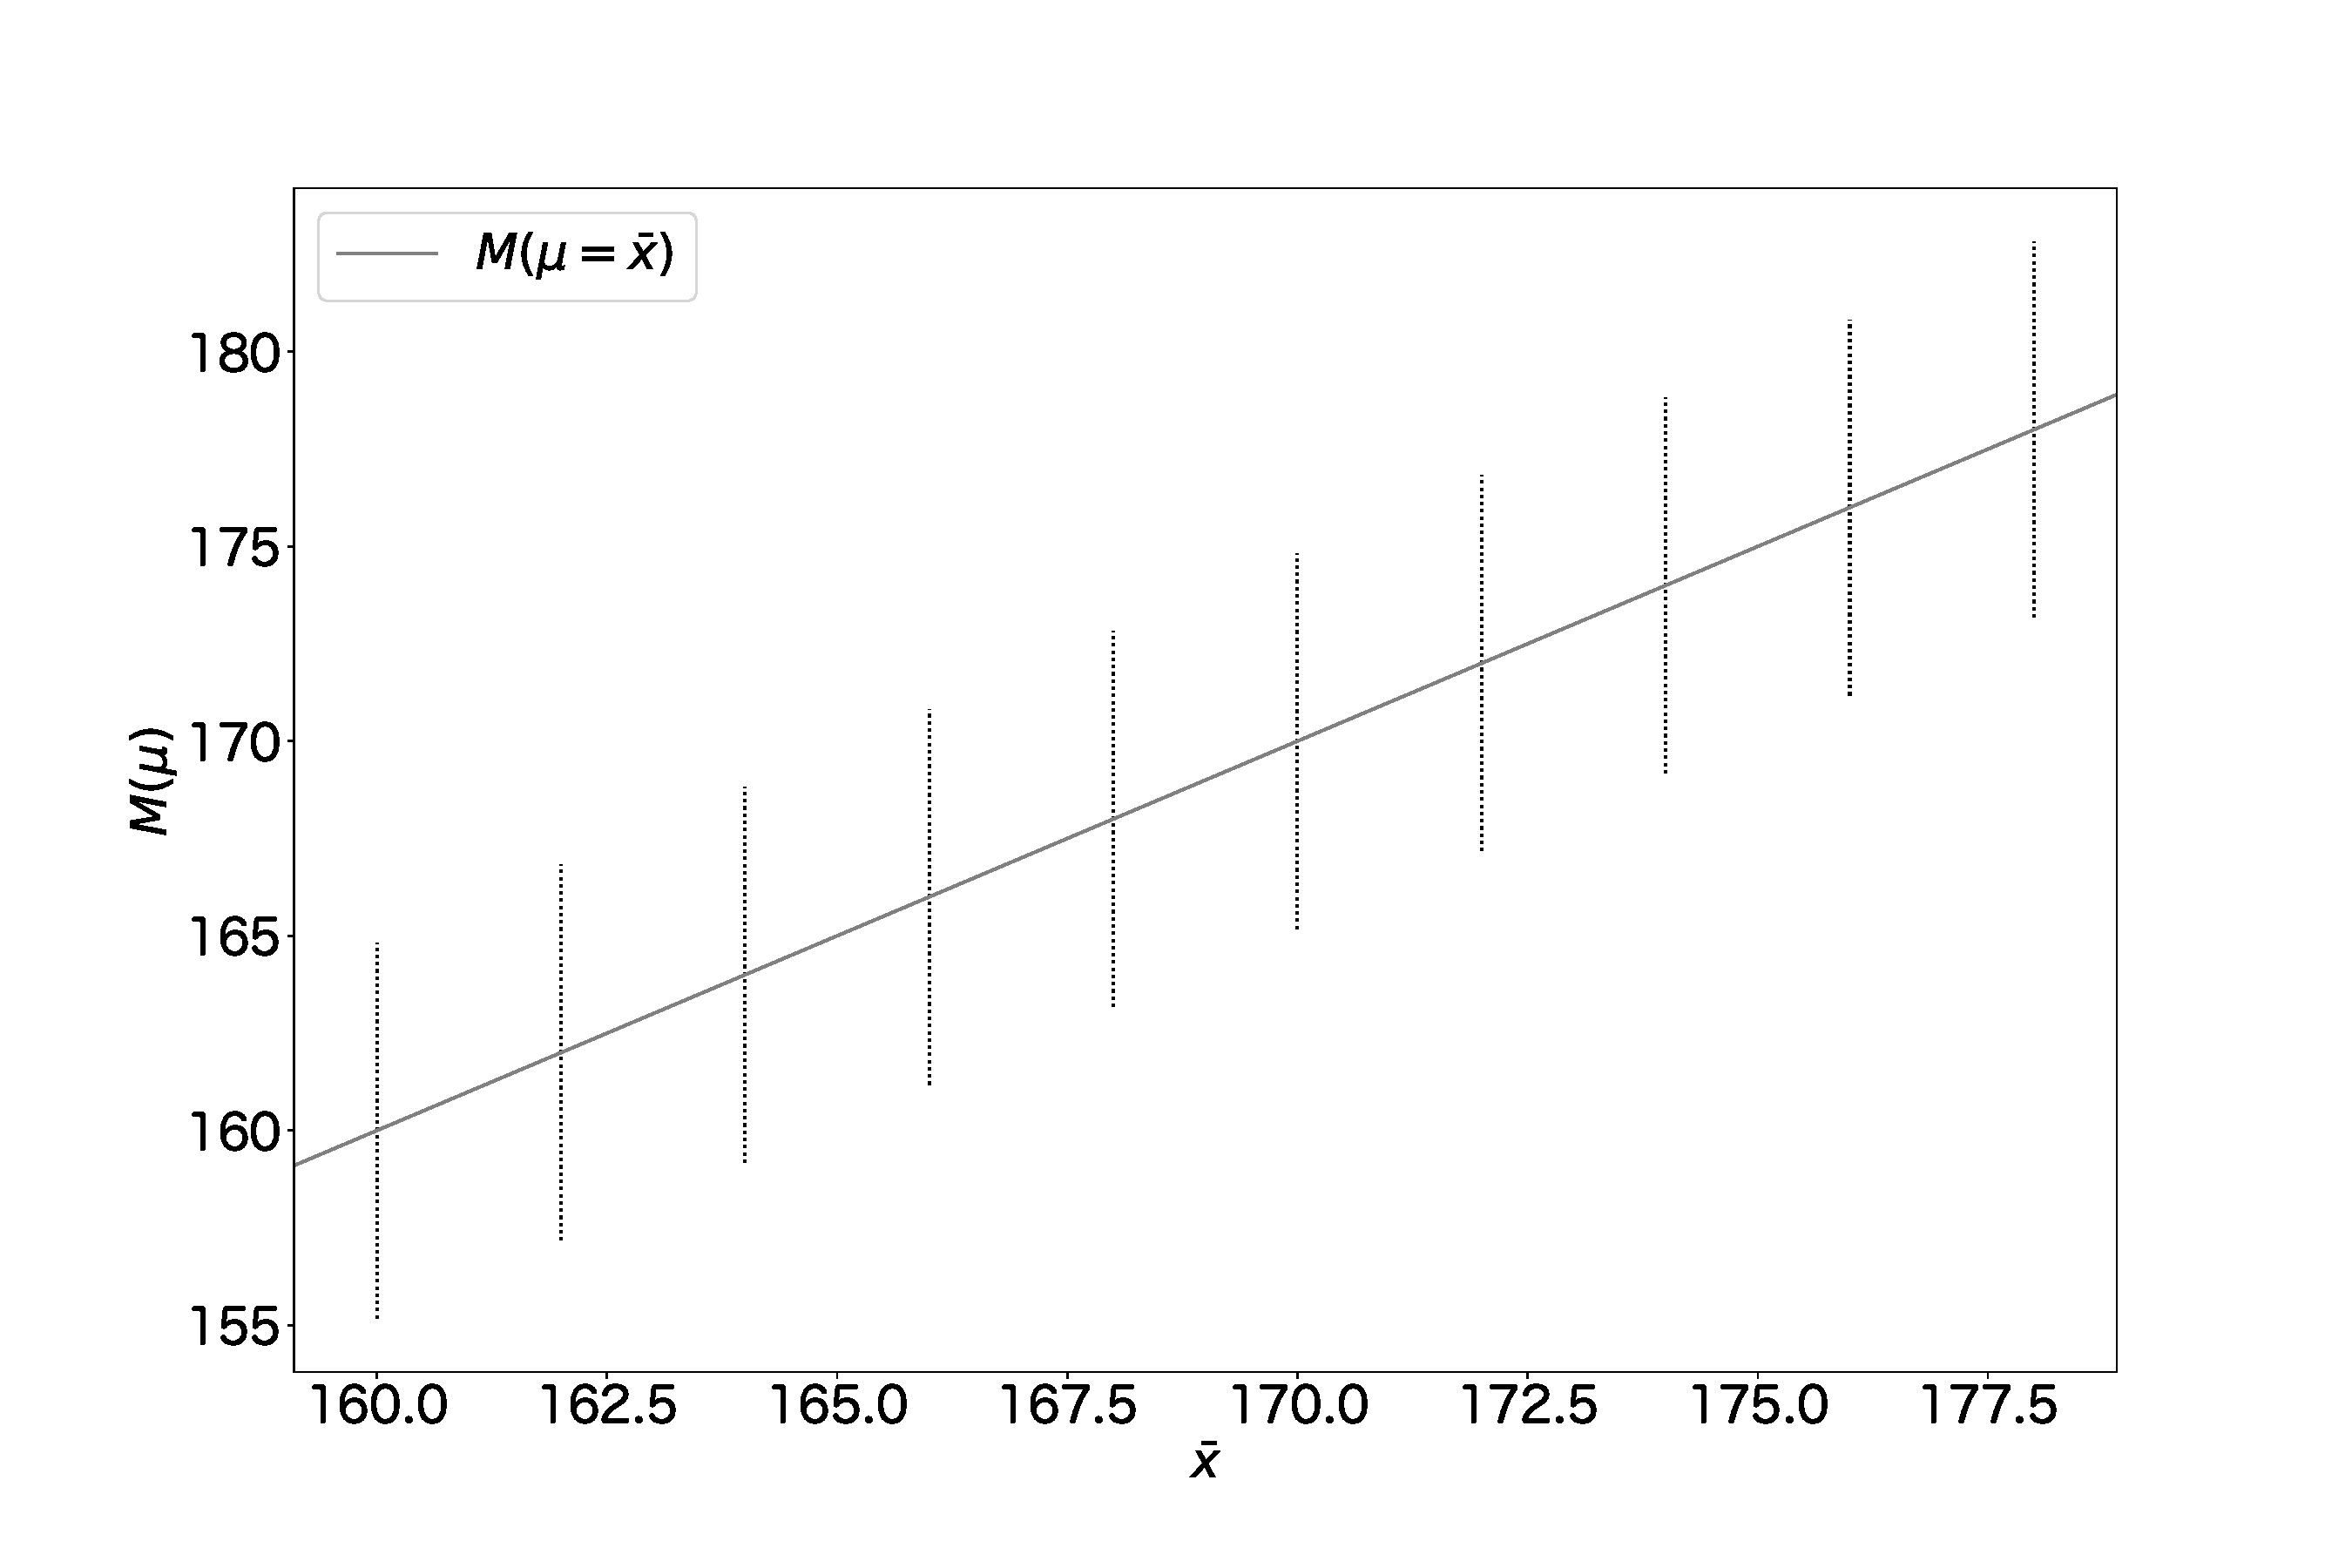
\includegraphics[width=15cm]{./image/04_/confidence_interval_model.pdf}
    %\caption{x軸は観測されたデータの平均値、y軸はモデルの母数$\mu$。}
  \end{center}
\end{figure}

\subsubsection{統計的仮説検定}
仮説検定はこれまで行ってきた統計モデルに対するモデルとの乖離を、たった一つの母数を対象に調べる方法です。
具体的には、データがある特定の母数$\mu$をもつ統計モデルの信頼区間に含まれるか否かによって、統計モデルが棄却されるかを調べます。
一般に、統計モデルの否定したい母数$\mu_0$を帰無仮説と言い、その母数ではないという$\mu\neq\mu_0$を対立かせつと言います。つまり、次のように帰無仮説を含む統計モデル$M_0$を構築します。
\begin{itemize}
    \item i.i.d
    \item 数学関数
    \item 統計モデルの母数を$\mu$とし、$\mu=\mu_0$
\end{itemize}
一番最後の仮説が帰無仮説と言います。
対立仮説を含む統計モデル$M_1$は、$M_0$と同様の仮説(1),(2)から構成されますが、仮設3は統計モデル$M_0$と$M_1$で異なります。
\begin{itemize}
    \item i.i.d
    \item 数学関数
    \item 統計モデルの母数を$\mu$とし、$\mu\neq\mu_0$
\end{itemize}
一番最後の仮説が対立仮説です。$M_1$の最後の仮説は、$M_0$の最後の仮設の否定系になります。

二つの統計モデルを作って、$M_0$で計算される信頼区間に、データから得られる統計量が入らないなら、$M_0$は棄却されます。逆に、統計量が信頼区間に入るなら、何も起こりません。
このように、否定したい仮説を設定し、少なくとも帰無仮説を含む統計モデルはだめだったと判断します。

\subsubsection{統計的仮説検定の手順}
統計的仮説検定の手順を確認します。
\begin{framed}
    \begin{enumerate}
        \item 過去の実験事実または予備実験から、無作為抽出したサンプルの出現頻度を予測する分布関数を特定する。ある点を中心に対称にデータが分布するのか、または、左右非対称にデータが分布するなどの知識・経験があったほうが良い。分布関数が全くわからないなら、正規分布を仮定する。
        \item その分布関数を含んだ統計モデルを構築する。統計モデルは以下の仮説から成り立つ。
        \begin{quote}
            \begin{itemize}
                \item 確率変数は独立同一分布に従う
                \item 分布関数
                \item 分布関数の母数がある値を取る
            \end{itemize}
        \end{quote}
        \item 統計モデルに母数を設定する.経験的に知っている値や、過去の論文や予備実験で明らかになった値である方が良い
        \item 統計モデルからサンプリングした確率変数の統計量が従う分布関数を探す。統計モデルの性質によって、母集団から得られた標本から得られた統計量の出現確率が計算可能になる。一般の仮説検定は本などでこの分布関数を確認する。
        \item 有意水準$\alpha$を設定する(さまざまな業界で$0.05$が設定される)。
        \item 母集団から無作為抽出を行い、標本を得る
        \item 標本が統計モデルにより推測できるかをもう一度考える。標本が統計モデルにより推測できること(標本の分布関数と統計モデルの分布関数がある程度一致している)、i.i.dであると考えることができるか。
        \begin{quote}
            標本が統計モデルにより推測できないと思われる場合、分布関数を変更し、統計モデルを再構築する。

            または、母集団の性質が別の分布関数になったのだから、仮説検定を使うまでもなく、変化があったことが主張可能である。例えば、正規分布で推測できると(過去の実験や研究結果から)思われてたデータが、実際には指数分布的だった場合など。この場合、計測機器・無作為抽出の方法などに異常がなかったかも確認すべきである。
        \end{quote}
        \item 標本が統計モデルによりよく推測できるなら、その統計量もなんらかの分布関数に従っているはずであると考えられる。標本から統計量を計算し、統計モデルの中で、その統計量がその値以上に大きな値をとる確率を計算する($p$値)。
        \item $p$値が$\alpha$以下であれば、統計モデルの仮説の中の少なくとも一つの仮説が現象と乖離していると考える。
        \item 仮説(1)のi.i.dと、仮説(2)の分布関数とが、計測事実と大きく乖離がないならば、設定した母数が現実を上手く推測できていないと考える。このとき、帰無仮説を含む統計モデルは絶対にだめなモデルと判断する。一般に、帰無仮説が棄却されると宣言する。統計モデルと現実に乖離があるなら、そのことを宣言するべきである。
        \item $p$が$\alpha$以上であっても、積極的に推測に使えるとは言わない。一般に対立仮説を採用するとは宣言しない。
    \end{enumerate}
\end{framed}


この手順を身長の検証をするためになぞってみます。
\begin{enumerate}
    \item 普段の観察から、身長はある平均値の周りに対象に分布していることがなんとなくわかっているので、対象な分布関数の中から関数を選ぶ。また、サンプルサイズが大きいときの標本を見ると、正規分布でよく推定できることが知られている。以上のことから、正規分布で推測を試みる。
    \item 次の統計モデルを構築する。
    \begin{quote}
        \begin{itemize}
            \item 確率変数は独立同一分布に従う
            \item 正規分布関数
            \item 正規分布関数の母数$\mu,\sigma=5.7$
        \end{itemize}
    \end{quote}
    \item $\mu=170$
    \item 次のことがわかっている$x_1,\cdots,x_n$が正規分布$N(\mu,\sigma^2)$に従う確率変数であるならば、$\frac{\bar{x}-\mu}{\frac{\sigma}{\sqrt{n}}}\sim N(0,1)$である。ここで、$\bar{x}=\frac{x_1+x_2+\cdots+x_n}{n}$
    \item $\alpha=0.05$
    \item 母数からサンプルをランダム抽出し、標本とする。
    \item 無作為抽出できていかたと、標本を正規分布で推測しても良さそうかを検証する
    \item 標本の平均$\bar{X}$を計算し、統計モデルでの出現頻度を計算する。
    \item $p<\alpha$ならば、統計モデルの仮定のうち少なくとも一つがデータと乖離していると考える
    \item 仮説(1),仮説(2)はそれほど悪くない仮説であると思われるので、母数に関する仮定が間違っていると考えられる。以上から、母数は$\mu$ではないと宣言する。
\end{enumerate}

もしも、予備実験から実験状況に変化がなければ、帰無仮説を含んだ統計モデルは棄却されにくい。実験状況に変化があれば、帰無仮説を含んだ統計モデルは棄却されやすくなる。

\subsubsection{他の書籍との対応}
一般の生物学の教科書には、以上の手順の一部が省略して書かれている。これは、特定の分布関数にデータが従っていることを前提にしているからであるが、そのようなケースは実際の現象においては非常に稀であると考えられる。ゆえに、データと想定した統計モデルの違い・一致を注意深く検証しながら、統計的仮説検定を利用することが求められる。
%統計モデルがデータと乖離していれば、推定値が何を意味するかが捉えられなくなるので、統計モデルの改訂を要求されることもある。
%ただし、$p$値を小さくすることを目標に統計モデルを改訂してはいけない。
\begin{framed}
    \begin{itemize}
        \item 帰無仮説($\mu = \mu_0$)・対立仮説($\mu\neq \mu_0$)を設定する(上記の1-3)。
        \item 仮説が正しいと考えたとき、検定統計量従う分布を考える(4)。
        \item $\alpha$を設定する。(5)
        \item 母集団からの無作為抽出により標本を得る。(6)
        \item 検定統計量を計算し、その出現する確率$p$値を計算する。それが$\alpha$以下であれば、$\mu=\mu_0$ではないと結論づける(帰無仮説が棄却された。)(7-10)
    \end{itemize}
\end{framed}



\begin{mybox}
    \begin{quotation}
    \paragraph{有意性検定・仮設検定}
    Fisherは、帰無仮説を含んだ統計モデルを設定し、モデルとデータの乖離を調べる枠組みを構築した。これを、有意性検定ということがある。これに対して、Newman-Pearsonらは、さらに、対立仮説を含んだ統計モデルを設定し、帰無仮説を含んだモデルとデータが乖離していた場合、対立仮説を含んだ統計モデルを採択すると言う立場をとった。これを、仮設検定と呼ぶことがある。現代の科学の多くは、FisherとNewman-Pearsonの両方を組み合わせ、帰無仮説・対立仮説を含んだ統計モデルを構築し、帰無仮説を含んだ統計モデルとデータの乖離を調べ、棄却されたとしても、対立仮説を含むモデルを積極的に採択することはない。

    %有意性検定を統計学\cite{upton2010統計学辞典,2009数理統計ハンドブック}や数学\cite{日本数学会2007岩波数学辞典}の辞書で調べたが、該当する言葉は見つからなかった。一方で、仮説検定は統計学\cite{upton2010統計学辞典,2009数理統計ハンドブック}などの辞書でも見つけることができた。
    %この言葉の使い方は、\cite{鳥類学における統計学_2018}に乗っていた。
    \end{quotation}
\end{mybox}


\begin{mybox}
    \begin{quotation}
\paragraph{正規分布を前提にできる場合}
TODO:意味不明\\
非常に限定された条件で、標本が正規分布していることを前提として使えます。具体的には、標本が分布関数(Cauchy分布は当てはまらない)により生成されていることが前提となる場合です。このとき、中心極限定理によって、十分なサンプルサイズがある場合には、データが正規分布に近づきます。
言い換えれば、サンプルサイズを増やしていけば任意に小さな$p$値を得ることができます。
一方で、一般の現象は特定の分布関数によってデータが生成されているとは言うことはできません。この場合、正規分布に近づくことが正当化できる科学理論はありません。     
    \end{quotation}
\end{mybox}


\begin{mybox}
    \begin{quotation}
    \paragraph{偶然の差が生じたかを確かめたい}
    「偶然の差が生じたかを確かめたい」や「こんなことが起こる確率は$5\%$くらい」という言葉を統計学の教科書で見たことがあると思います。これはそれぞれ、「統計モデルの上で統計量が現れる確率が十分小さいことを確かめたい」や「統計モデル上でそのような統計量が得られる確率が$5\%$」を省略して書いたものです。
    
    統計学では、実験で得られたデータは、同様の実験を行った場合、同様のものが得られるということが要求されます。このことを現象に再現性があると言います。再現性のないデータを現状の統計学で扱うことはかなり難しい課題であり、現実の現象が得られる確率を議論することは困難です。
    \end{quotation}
    \end{mybox}
    
    
    \begin{mybox}
    \begin{quotation}
    \paragraph{帰無仮説のもとで偶然には起こり得ないことが起こった}
    帰無仮説のもとで偶然には起こり得ないことが起こったと言うふうに書くと、現実に起こりにくいと言うふうに印象付けられてしまう。非現実である統計モデルの上で、実験で得られた統計量以上の値が得られる確率は十分小さいと言い換えた方が良い。
    \end{quotation}
    \end{mybox}
    

\subsection{検出力}
母数の異なる二つの統計モデル$M_a,M_b$について考察する。母数から標本を得て、それぞれの統計モデルを統計量を元に評価する。
\subsubsection{検出力の定義}
$M_a$を棄却する判断をする閾値は、言い換えると、統計モデル$M_a$の棄却される母数(棄却域$R$)の出現確率を$\alpha$と言った。
また、$M_a$の棄却できない母数の範囲(信頼区間$A$)に$M_b$の統計量が存在する確率を$\beta$とする。$\beta$を検出力という\footnote{検出力を検定力または統計力と呼ぶこともある。\url{https://id.fnshr.info/2014/12/17/stats-done-wrong-03/}}。
$\alpha$は統計モデルとデータを比較したとき、そのモデルを棄却する指標である。
$\beta$は、二つの異なるモデルを比較するための指標で、一方のモデルで棄却できない母数がもう一方のモデルで出現する確率である。
$M_a$に対する$M_a$の検出力は、$1-\alpha$であり、$M_a$を棄却する閾値を低く設定すると、$\beta$は大きな値になる。
二つの統計モデルの母数がよく一致するならば、$\beta$は$1-\alpha$に近い値を取り、一致していないならば、$\beta$は0に近い値を取る。
具体的に、式で書くと、
\begin{eqnarray*}
    P_a(\mu \in R_a) = \alpha\\
    P_b(\mu \in A_a) = \beta
\end{eqnarray*}
ここで、$R_a,A_a$はそれぞれ統計モデル$M_a$の棄却域、信頼区間、$P_a,P_b$は、それぞれ統計モデル$M_a,M_b$における統計量の確率密度関数。

\subsubsection{正規分布モデルの検出力}
具体的に、$P_a(\mu \in R_a),P_b(\mu\in A_a)$を計算してみる。
正規分布を含む統計モデルを構築する
\begin{quote}
    \begin{enumerate}[(1)]
\item i.i.d
\item $N(\mu,\sigma^2)$
\item 母数$\mu$,$\sigma$は既知とする(一般性を持たせるために、具体的な値は書かない。$\sigma=1$と読み替えて進めても良い)
\end{enumerate}
\end{quote}
このモデルを$M(\mu)$とし、$M_a=M(\mu_a),M_b=M(\mu_b)$とする。
$M_a$または、$M_b$からサンプリングされた確率変数$x_1,x_2,\cdots,x_n$の平均値は、それぞれ$\bar{x}_a\sim N(\mu_a,\sigma/n)$または$\bar{x}_b\sim N(\mu_b,\sigma/n)$である。
$M_a$の信頼区間$A_a$は、$|\bar{x}_a|<\mu_a+\sigma / \sqrt{n}z_{2.5\%}$である。
このとき、$P_a$を$N(\mu_a,\sigma)$の確率密度関数とすると、
\begin{equation*}
    P_a(\mu \in A_a) = \alpha
\end{equation*}
であるのは定義から明らか。
また、$P_b$を$N(\mu_b,\sigma)$の確率密度関数とすると、
\begin{equation*}
    P_b(\mu \in A_a ) = \beta
\end{equation*}
である。
$\mu_a$と、$\mu_b$が一致していれば、$P_b(\mu \in A_a ) = 1-\alpha$である。
$\mu_b$が$\mu_a$から離れていくと、$P_b(\mu \in A_a)=0$に近づいていく。


\begin{figure}
\begin{center}
    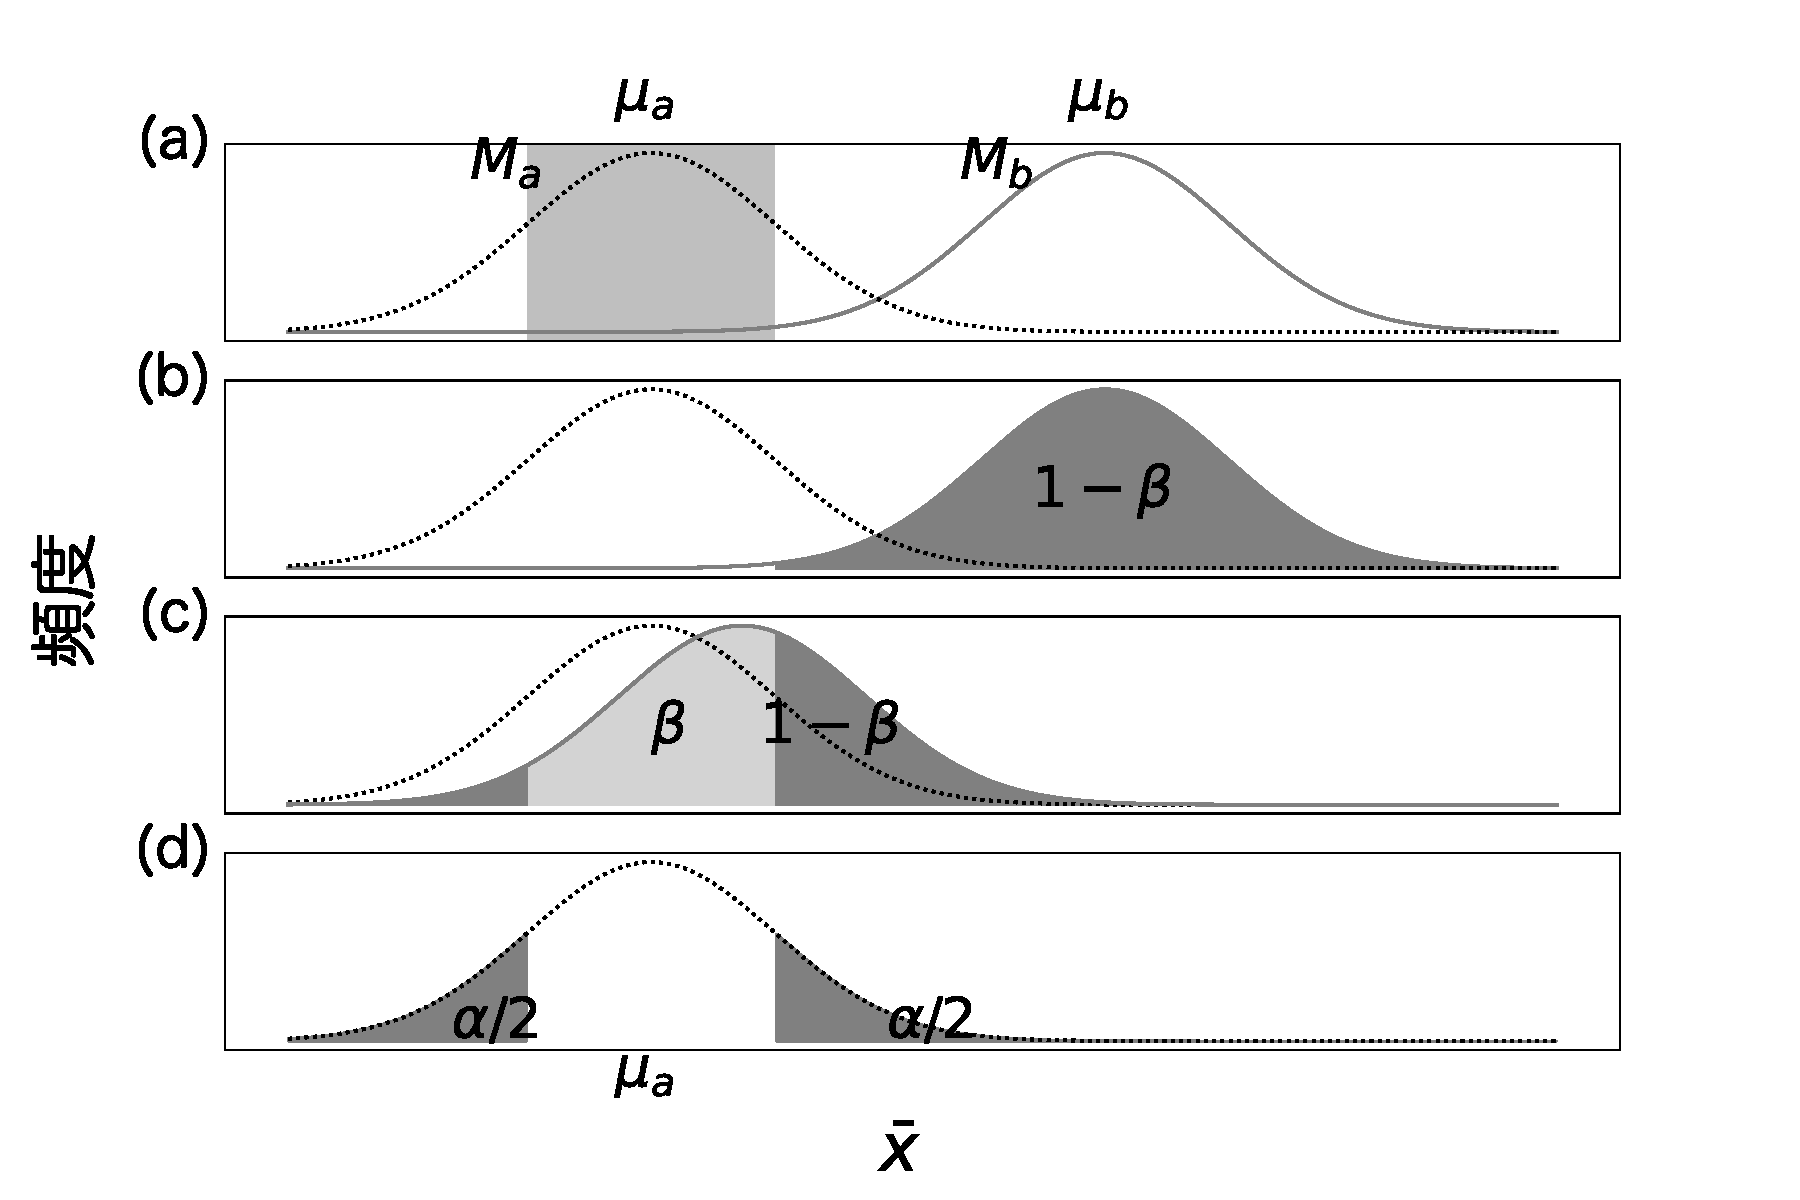
\includegraphics[width=15cm]{./image/04_/power_of_a_test_2.pdf}
    \caption{統計モデル$M_a,M_b$から計算された統計量$\bar{x}$の確率分布$P_a,P_b$。(a)灰色の範囲は$M_a$の信頼区間。(b)灰色の領域は、$1-\beta$の領域を示している。$\beta$の領域が小さいので、描画できなかった (c)$\mu_b$が$\mu_a$に近いときの$\beta$と$1-\beta$の領域。(d)灰色の範囲の面積が$\alpha$を示している。}
    \label{fig:power_of_test_alpha_beta}
\end{center}
\end{figure}


検出力と$\alpha$の領域を図示した(図\ref{fig:power_of_test_alpha_beta})。$M_a$の$95\%$信頼区間は、$|\mu|<\mu_a+z_{0.025}\frac{\sigma}{\sqrt{N}}$である。信頼区間は、図\ref{fig:power_of_test_alpha_beta}(a)において灰色で塗った$x$軸の範囲である。$\alpha$は図\ref{fig:power_of_test_alpha_beta}(c)の灰色で塗りつぶした領域の面積である。
検出力$1-\beta$は、$M_b$における$M_a$の信頼区間の外側の領域の面積なので、図\ref{fig:power_of_test_alpha_beta}(b)の濃い灰色の範囲である。

$\alpha$を0に近づけていくと、信頼区間は徐々に大きくなり、$\beta$は大きくなる。
$\alpha$を1に近づけていくと、信頼区間は徐々に狭くなり、$\beta$は小さくなる。



\begin{figure}
    \begin{center}
        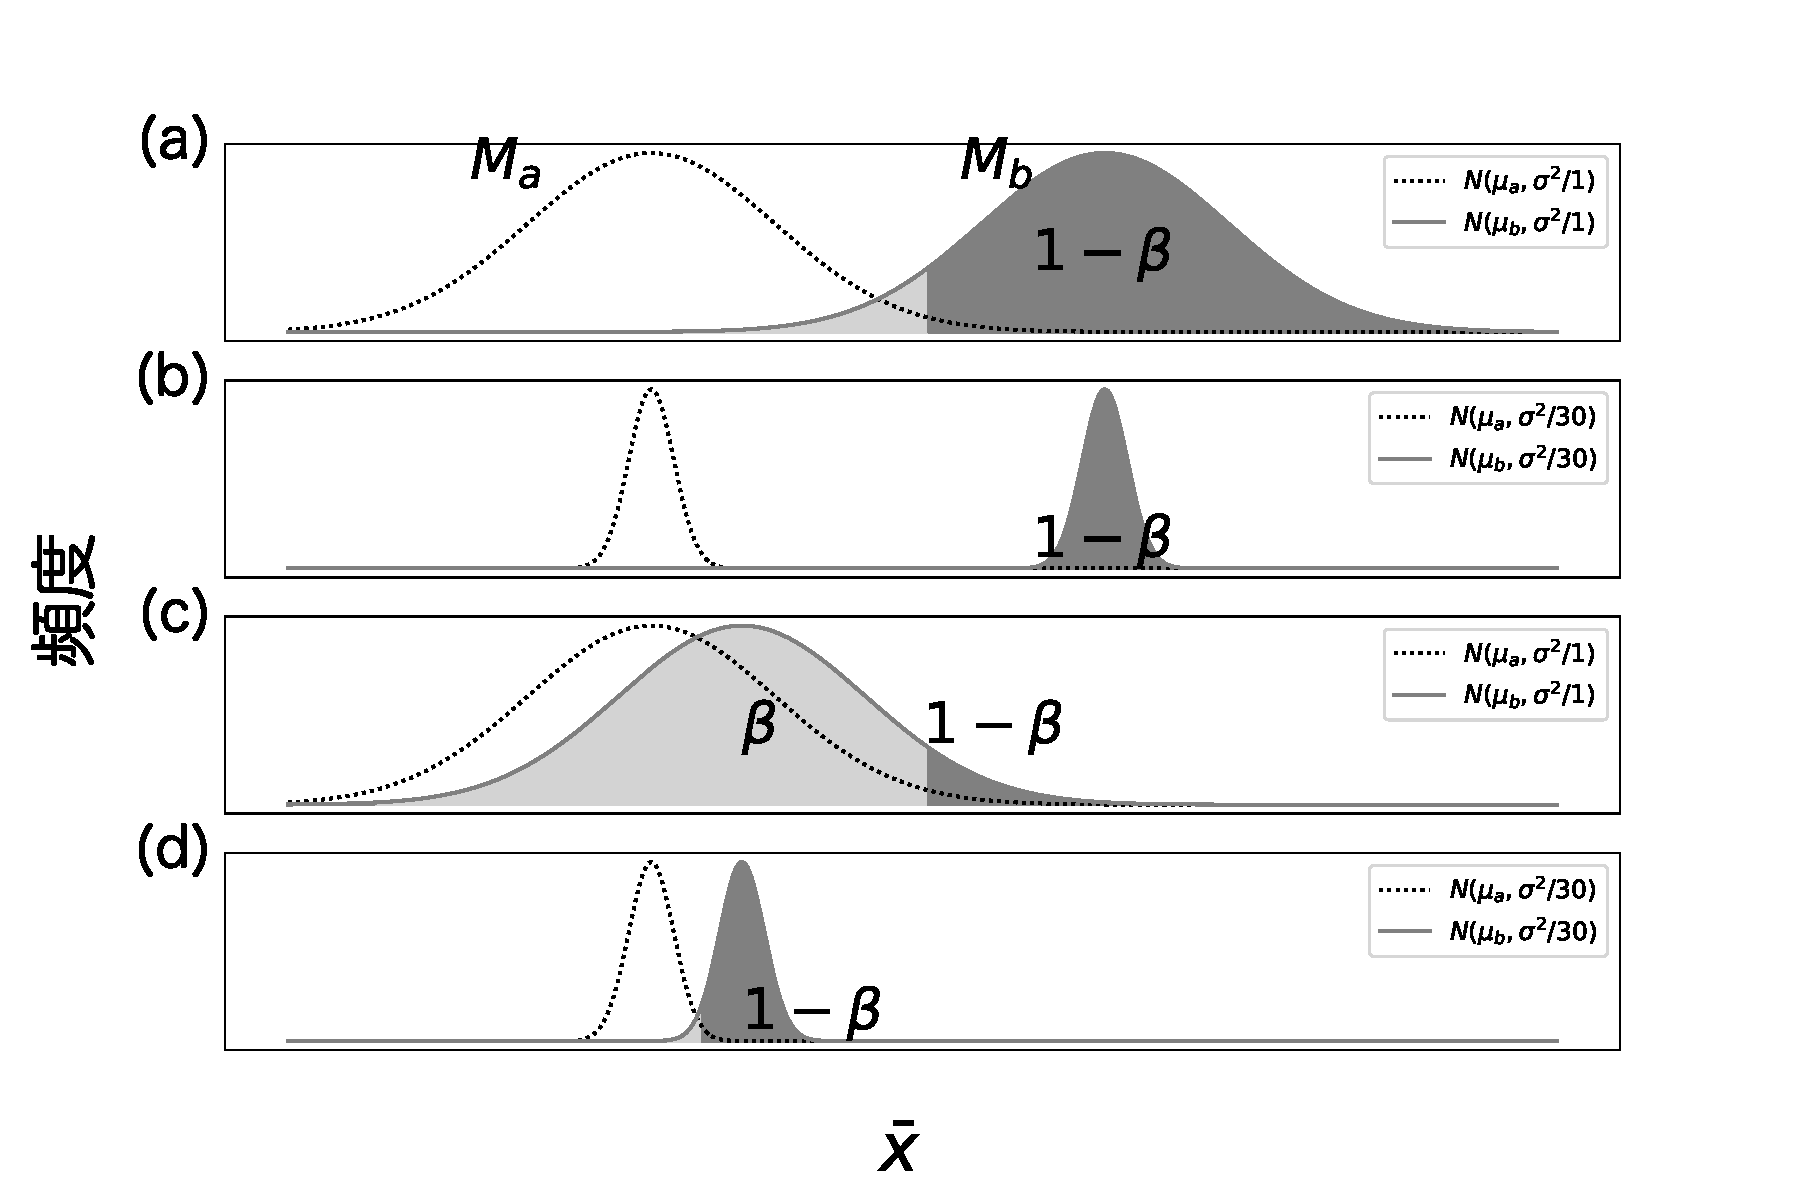
\includegraphics[width=15cm]{./image/04_/power_of_a_test_3.pdf}
        \caption{統計モデル$M_a,M_b$から計算された統計量$\bar{x}$の確率分布$P_a,P_b$。(a)$\mu_a,\mu_b$のサンプルサイズ$1$の平均値がしたがう確率密度関数$N(\mu_a,\sigma^2/1),N(\mu_a,\sigma^2/1)$。(b)(a)と同じ$\mu_a,\mu_b$に対して、サンプルサイズを$30$にした場合の確率密度関数。(c)$\mu_a,\mu_b$が(a)よりも近いときの$\bar{x}$の確率密度関数。(d)(c)と同じ$\mu_a,\mu_b$に対してサンプルサイズを$30$にした場合の$\bar{x}$の確率密度関数。}
        \label{fig:power_of_test_alpha_beta_sample_size}
    \end{center}
    \end{figure}

    

$\alpha$、$M_a$の母数$\mu_a$、$M_b$の母数$\mu_b$を固定したまま、サンプルサイズを変化させるときのことを考えてみる(図\ref{fig:power_of_test_alpha_beta_sample_size})。$\bar{x}$の確率密度関数($N(\mu,\sigma^2/n)$)の分散がサンプルサイズによって変化することは明らかである。このことから、サンプルサイズが大きくなると、信頼区間は徐々に狭くなり、$1-\beta$は大きくなる。サンプルサイズが小さいときは、$1-\beta$も小さくなる。

$\mu_a$を固定し、$\mu_b$を変化させたときの検出力$1-\beta$を図\ref{fig:power_of_test_N_mu0_variable}に示した。
サンプルサイズが大きければ、$1-\beta$も大きくなることがわかる。

\begin{figure}
    \begin{center}
        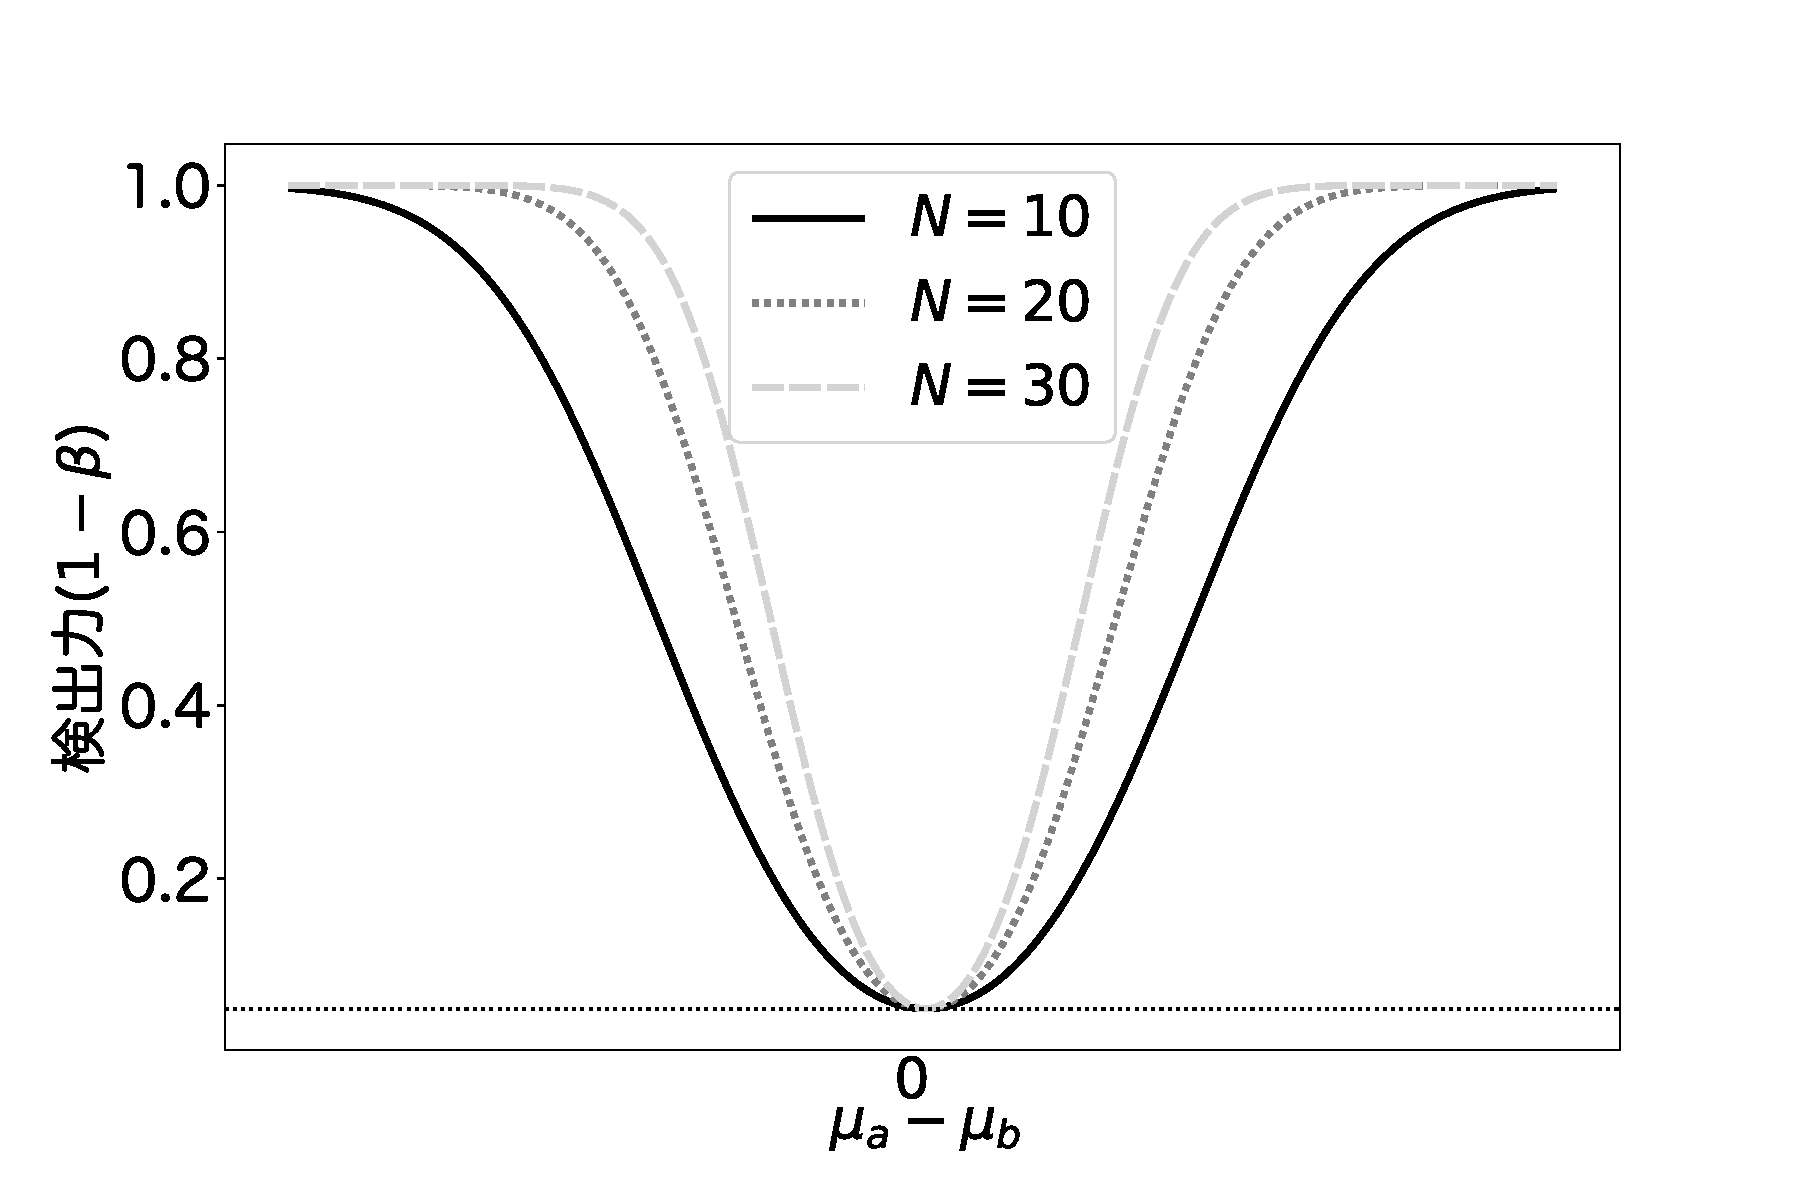
\includegraphics[width=15cm]{./image/04_/power_of_test.pdf}
        \label{fig:power_of_test_N_mu0_variable}
        \caption{$\mu_a$を変数にしたときの検出力(検出力関数)。}
    \end{center}
\end{figure}

$\beta$を定義したことにより、$M_a,M_b$の違いをはっきりさせるために必要なサンプルのサイズが計算できる。ここでは、$\mu_a,\mu_b$が固定されている状況を考える。
検出力$1-\beta$は$1$に近いほど、$M_a,M_b$が違うと主張できる。
あらかじめ決めたおいた基準の$1-\beta$を閾値を設定し、それ以上の$1-\beta$となるサンプルサイズを計算すれば良い。
サンプルサイズが小さければ、$M_a$と$M_b$の違いは曖昧であり、サンプルサイズが大きくなると、はっきりとモデルの違いがわかる。



\begin{mybox}
    \begin{quote}
    \paragraph{第一の過誤・第二の過誤・統計モデルが正しい}
        Neyman-Pearson流の統計学の方言においては、$\alpha,\beta$を次のように定義する。帰無仮説を含む統計モデルが正しいとき、誤ってそのモデルを棄却してしまう間違いを第一の過誤といい、この確率を$\alpha$とする。また、対立仮説を含む統計モデルが正しいのに、帰無仮説を採択する間違いを第二の過誤といい、この確率を$\beta$とする。

        Fisher流派とNeyman-Pearson流派の両方を同じように扱うことが問題視されている[\cite{published_papers/18436201}]。
        私は、ある統計モデルが正しいとは考えないので、「モデルが正しいとき、間違えてそのモデルを棄却する間違い」ということを考える流派に同意できなかった。
        統計モデルは棄却されることはあるが、正しいことや積極的に採択されることは稀であるというのはFisherの流派が近いように思う。
        ただし、Fisherは、「$p$値を帰無仮説が正しいという条件のもとで、手元にあるデータ、およびさらに極端なデータが得られる確率」と定義した[\cite{1573106361610039296}]。
        ここでの正しいという言葉の意図が重要である。
        私は、「統計モデルの仮説が自然を記述するのにほどほど良いと考えられるとき、手元にあるデータの統計量以上の隔たりが統計モデル内で得られる確率」という意味であると考えている。

        Neyman-Pearson流派の統計学の教科書を科学の分野で見つけることができていない。
        Fisher流派とNeyman-Pearson流派の両方を書いている教科書は存在しているが、「帰無仮説を含む統計モデルが正しい」とはどういうことかを答えたものを見つけることができていない。
    \end{quote}
\end{mybox}

\begin{mybox}
    \begin{quote}
    \paragraph{正解と回答の違い}
    回答がYesまたはNoである問題において、回答がYesな問題に、Yesと答えることを、True Positiveといい、Noと答えることをFalse Negativeという。回答がNoな問題に、Yesと答えることを、False Positive、また、Noと答えることをTrue negativeという。
        \if 0
    \begin{table}[hbtp]
        \caption{$\sigma$を基準にした値の出やすさ}
        %\label{table:data_type}
        \centering
        \begin{tabular}{ccc}
            \hline
            aa  & 陽性  &  陰性 \\
            \hline \hline
            陽性 & 真陽性 & 偽陽性  \\
            陰性 & 偽陰性 & 真陰性\\
        \end{tabular}
    \end{table}
    \fi
    \end{quote}
\end{mybox}


\begin{mybox}
    \begin{quote}
    \paragraph{過誤の概念}
    第一の過誤・第二の過誤に関する批判として\cite{norleans2004臨床試験のための統計的方法}がある。
    \cite{2010毒性試験に用いる統計解析法の動向}において引用されていた部分を引用しておく。私も彼らの意見に同意する。


    過誤の概念は非現実的である。根本的な問題は、我々が真実を知らないことである。現実の臨床試験では、我々は実験から学び、真実を知りたいと願うのであって、真実がすでに知られており、我々の観察を判断するのに利用できる、というようなものではない。現在利用できる情報だけに基づく決定は、それ以上の情報が利用できるときには間違っていたことがわかることもあり得る。それ以上の情報が得られないとき、決定を行なった元になる情報でその決定の評価を行うことは理論的に不可能である。一つの試験では、試験さそのものから得られる情報が、利用できる唯一の情報である。利用できる情報の調査と競合する利害の注意深いバランスを考慮した後でのみ、仮説の棄却や採択の判断が行われる。その後の試験の情報が利用できるようになるまでは、現在の判断が正しいか誤りかを判断する情報は存在しない。従って、一つの試験にとっては、過誤の考え方は全く意味を持たない。
    \end{quote}
\end{mybox}

\begin{mybox}
    \begin{quote}
    \paragraph{p値の多様な解釈}
$p$値は分野によって多様な解釈がなされることがある\cite{published_papers/18436201,2020医療統計解析使いこなし実践ガイド}。
\if 0
例えば、ASAの声明[\cite{ASA_JA}]を引用しているにもかかわらず、
$p$値は、証明したい仮説が真である場合、研究で行った前提条件が担保されている場合、研究で得られた結果が実際に得られる確率を示している\cite{2020医療統計解析使いこなし実践ガイド}。

などと書かれる場合がある。
ここで、「実際に得られる確率」が何を指しているのかが不明確であるが、「統計モデル上で実験で得られた統計量が得られる確率」を意図すると読み替えることはできるのだろうか。
\fi

よい解釈として以下の6つの原則が示されている\cite{published_papers/18436201}
\begin{enumerate}
    \item $p$値はデータと特定のモデルが矛盾する程度を示す指標の一つである。
    \item $p$値は調べている仮説が正しい確率や、データが偶然飲みで得られた確率を図るものではない。
    \item 科学的な結論や、ビジネス、政策における決定は$p$値がある値を越えたかどうかのみに基づくべきではない。
    \item 適正な推測のためには、全てを報告する透明性が必要である
    \item $p$値や統計的優位性は、効果の大きさや結果の重要性を意味しない。
    \item $p$値は、それだけでは統計モデルや仮説に関するエビデンスの、よい指標とはならない。
\end{enumerate}

    $p$値や信頼区間を報告することがASAの声明では求められている。私は、それら以外の情報として、ランダムサンプリングされているということ・再現可能性・正規分布を含んだ統計モデルなどを研究者がどの程度信じているのかということも報告するべきだと考えている。統計モデルの仮定が現象から著しく外れているのならば、統計モデルを使った推論は無意味である。
    また、研究者の統計学への心情がわかれば、報告に価値があることを理解しやすくなる。

    誤解とされる解釈はも引用しておく\cite{idiot_statistics2014}\footnote{原典は\cite{GOODMAN2008135}である。孫引き引用である}。
    \begin{enumerate}
        \item $p=0.05$ならば、帰無仮説が真である確率は$5\%$しかない。
        \item $p\geq 0.05$のような有意でない結果は、グループ間に差がないことを意味する
        \item 統計的に有意な発見は客観的に重要である
        \item $p$値が$0.05$より大きい研究と小さい研究は矛盾する
        \item $p$値が同じ研究は帰無仮説に対して同等の証拠を提供する。
        \item $p=0.05$は、帰無仮説のもとで$5\%$しか起こり得ないデータを観察したことを意味する
        \item $p=0.05$と$p\leq 0.05$は同じことである。
        \item $p$値は不等式の形で書かれるものである(例えば、$p=0.015$のときは$p\leq 0.02$とする)。
        \item $p=0.05$は、帰無仮説を棄却したとしたら、第一種の誤りの確率が$5\%$しかないことを示す。
        \item 有意水準$p=0.05$のもとで、第一種の誤りの確率は$5\%$になる。
        \item ある方向を向いた結果やその方向の結果があり得ない差異を気に留めないのであれば、片側の$p$値を用いるべきである。
        \item 科学に関する結果や処方の方針は$p$値が有意であるかどうかに基づくべきである。
    \end{enumerate}

    \end{quote}
\end{mybox}

\subsubsection{$\beta$の計算}
正規分布を含んだ統計モデル$M_a,M_b$を使って、$\beta$を計算してみる。
$M_a$の信頼区間は、
\begin{equation*}
    -z_{0.025}\leq \frac{\sqrt{n}(\bar{x}-\mu_a)}{\sigma}\leq z_{0.025}
\end{equation*}
より、
\begin{equation*}
    A_a = \{ \mu ; \mu_a -\frac{\sigma}{\sqrt{n}}z_{0.025} \leq \mu \leq \mu_a +\frac{\sigma}{\sqrt{n}}z_{0.025} \}
\end{equation*}
である。ここで、$a=\mu_a -\frac{\sigma}{\sqrt{n}}z_{0.025},b = \mu_a +\frac{\sigma}{\sqrt{n}}z_{0.025} $とおく。棄却域は$A_a$以外の$\mu$である。$M_b$の標本平均$\bar{x}_b$は、$N(\mu,\frac{\sigma^2}{n})$に従うので、$A_a$の区間で、$N(\mu_b,\frac{\sigma^2}{n})$の面積を計算すれば良い。
ここで、$\frac{\sqrt{n}(\bar{x}_b-\mu_b)}{\sigma}\sim N(0,1)$である。
このことを利用すると、
$a,b$は、$N(\mu_b,\frac{\sigma^2}{n})$の確率変数だとすると、
\begin{eqnarray*}
    A &=& \frac{\sqrt{n}(a-\mu_b)}{\sigma} \\
    &=& \frac{\sqrt{n}(\mu_a-\frac{\sigma}{\sqrt{n} z_{\alpha/2}})}{\sigma}\\
    &=& -z_{\alpha/2}+\frac{\sqrt{n}}{\sigma}(\mu_a-\mu_b)
\end{eqnarray*}
同様に、
\begin{eqnarray*}
    B &=& \frac{\sqrt{n}(b-\mu_b)}{\sigma} \\
    &=& \frac{\sqrt{n}(\mu_a-\frac{\sigma}{\sqrt{n} z_{\alpha/2}})}{\sigma}\\
    &=& z_{\alpha/2}+\frac{\sqrt{n}}{\sigma}(\mu_a-\mu_b)
\end{eqnarray*}
である。以上より、確率密度関数$N(0,1)$において、$-z_{\alpha/2}+\frac{\sqrt{n}}{\sigma}(\mu_a-\mu_b) \leq x\leq  z_{\alpha/2}+\frac{\sqrt{n}}{\sigma}(\mu_a-\mu_b)$の間で積分すれば良い。

$d=\frac{\mu_a-\mu_b}{\sigma}$とおく。$d=0.6,n=9$とする。このときの$\beta$を計算してみる。$N(0,1)$において、$-z_{\alpha/2} -0.6\sqrt{n} \leq x \leq z_{\alpha/2} +0.6\sqrt{n}$の区間で積分する。

\begin{lstlisting}
A,B = norm.interval(0.95,0.,1)
N = 9
d = 0.6
a,b = A+d*np.sqrt(N),B+d*np.sqrt(N)
print(a,b)
norm.cdf(b,0,1)-norm.cdf(a,0,1)
\end{lstlisting}

答えは、$0.564$

\subsubsection{データを元にしたモデルとモデルの類似度}
統計モデルAを$M(\mu=170)$とし、統計モデルBを$M(\bar{X})$とする。ここで、$\bar{X}$は、無作為抽出によって得られた標本の平均であり、標本の大きさを$100$とする。
モデルA,Bの間の検出力が計算可能である。
$d=\frac{170-\bar{X}}{6.8}$、$n=100$であるので、$\bar{X}=168$を得たとすると、
\begin{lstlisting}
A,B = norm.interval(0.95,0,1)
N = 100
d = (170-168)/(6.8)
a,b = A+d*np.sqrt(N),B+d*np.sqrt(N)
print(a,b)
norm.cdf(b,0,1)-norm.cdf(a,0,1)
\end{lstlisting}
その検出力は、$0.163$

\subsubsection{サンプルサイズ}
$d$と検出力を指定したときに、$M_a,M_b$の類似度を検出力以上にするためのサンプルサイズが計算できる。
$\beta=0.1,\d=0.8$とし、この$\beta$を満たすように$N$を計算した。

\begin{lstlisting}
A,B = norm.interval(0.95,0.,1)
beta = 0.1
d = 0.8
for N in range(10,200,2):
    a,b = A+d*np.sqrt(N),B+d*np.sqrt(N)
    beta_ = norm.cdf(b,0,1)-norm.cdf(a,0,1)
    if beta_ < beta:
        break
print(N)
\end{lstlisting}
計算を実行すると、$18$であることがわかる。


\subsection{第一の過誤}
統計モデルの中で、統計モデルを統計量により検査するときに、モデル自身を絶対にダメなモデルと判断してしまうことを第一の過誤(type I error)と言う。
この過誤は、2つの要因に分解すると\footnote{$\alpha_2$は$\alpha_1$に関係するので実際には、分解できない。}、不適切な統計量を使用することで、棄却域と統計量の違いにより生じる$\alpha_1$、そして、検定を繰り返して生じる$\alpha_2$である($0<\alpha_1+\alpha_2 \leq 1$)。
$\alpha_1+\alpha_2=\alpha$となっていれば、有意水準$\alpha$の検定ができる。
$\alpha_1$は、統計モデルと、その統計量の関数になっており、言い換えれば、統計モデルと統計量の適合度を測る指標である。
正規分布を含んでいる統計モデルを使い、統計量$T$を使った場合、$\alpha_1 \approx	 0 $であるが、指数分布を含んだ統計モデルを使い、統計量$T$を使った場合、$\alpha_1 > 0$となる。これを見ていく。
$\alpha_2$については、後で調べる。
$\alpha_2$は、$\alpha\times 2$以上になる場合、軽視されることはないが、
$\alpha_1$が同程度の隔たりになる場合においては無視され、$\alpha_1$は$\alpha_2$よりも軽視されがちである。
%統計モデルに対して不適切な統計量を使ってモデルの検証を試みると、第一の過誤が変化することがわかっている。

\subsubsection{どんな統計モデルでも$T$統計量で調べよう($\alpha_1$)}
統計モデルの分布の仮定が正規分布以外の場合においても、$T$統計量を使ってモデル自身を検証できるのかを調べる。次の統計モデル$M(\lambda)$を構築する。
\begin{enumerate}
    \item $X_1,X_2,\cdots,X_n $はi.i.d
    \item 指数分布
    \item $\lambda$
\end{enumerate}
母数$\lambda=1$とした統計モデルを$M(1)$とする。
$M(1)$からランダムサンプリングした確率変数$x_1,x_2,\cdots,x_n$から次の統計量を計算する。
\begin{equation*}
    T = \frac{\bar{X}-1}{\sqrt{\frac{\sigma^2}{n}}}
\end{equation*}
ここで、$T \sim t(n-1)$とする。
$T$値が$t(n-1)$の棄却域に入っている頻度を数値計算により計算する。
具体的に、平均$1$の指数分布または、平均$1$、標準偏差$1$の正規分布からサンプルを得て標本を作る。その標本を$100000$回取得する。
このとき、$T$値を計算し、$T$値いじょの値が得られる確率$p$を計算する。その$p$が$p<0.05$となる割合を計算する。以上をサンプルサイズを変化させてシミュレーションを行なった。
平均$1$、標準偏差$1$の正規分布の場合、$T$値は$t(n)$分布に従ので、$p<0.05$となる頻度も、$5\%$程度になることが期待される。
一方で、平均$1$の指数分布の場合、$T$は$t(n-1)$分布に従うとはいえない。このことから、$p<0.05$となる頻度は計算してみなければわからない。


\begin{figure}
    \begin{center}
        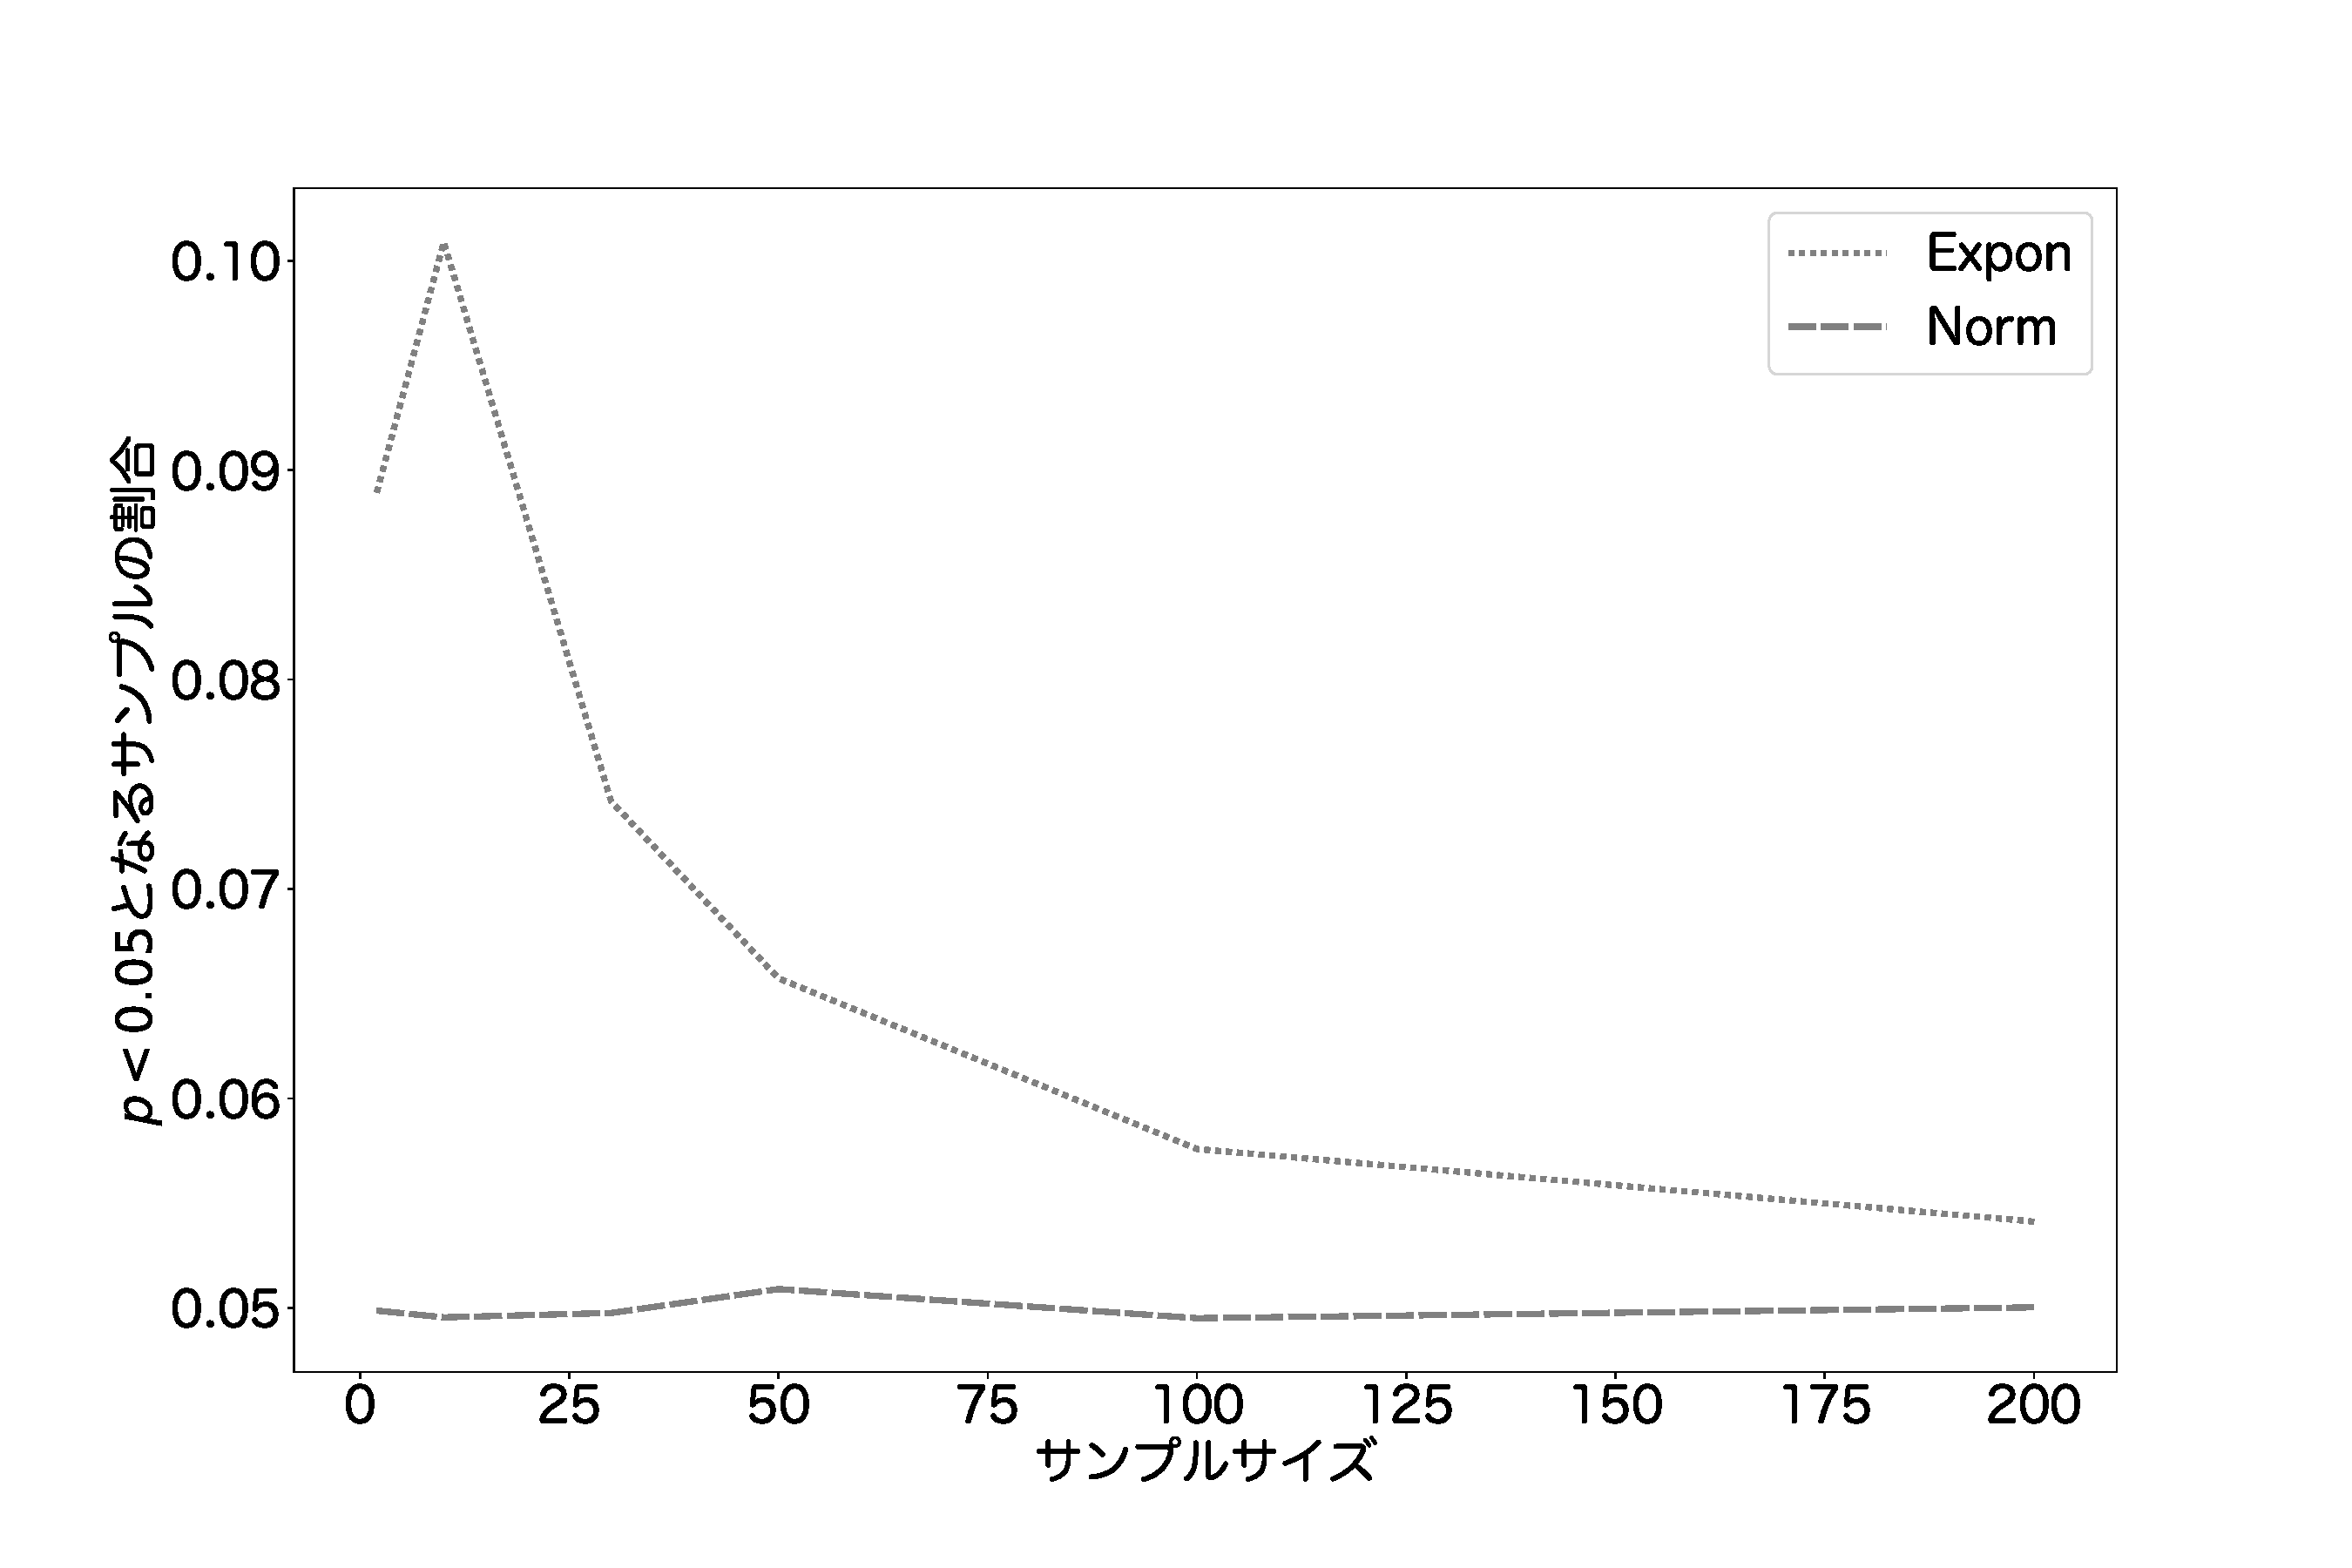
\includegraphics[width=15cm]{./image/04_/t_test_expon_norm.pdf}
        \caption{正規分布または指数ぶんぷから得た標本の$T$値から計算した$p$値で、$p<0.05$以下になる割合}
    \end{center}
\end{figure}

シミュレーションの結果、正規分布から標本を得た場合、$p<0.05$になる割合は、サンプルサイズに依存せず、$5\%$程度であり、期待通りである。
一方で、指数分布から標本を得た場合、$p<0.05$になる割合はサンプルサイズに応じて変化しており、また、どのサンプルサイズでも$p<0.05$となる割合は$5\%$より多い。

このことから、指数分布を含んだ統計モデルの$\alpha_1$は、$\alpha_1>0.05$であることがわかり、統計量を正しく選ばなかったことで、第一の過誤が期待した$0.05$よりも大きくなっていることがわかる。

\if 0
\subsubsection{いつでも正規分布を含んだ統計モデルでいこう}
データが非対称に分布しているのに、統計モデルに正規分布を指定した場合、推定が正しく行えないことを確認しておこう\footnote{元ネタ。
    小標本 t 検定の誤解:中心極限定理と一般化線形モデル 井口豊(生物科学研究所,長野県岡谷市)\url{https://biolab.sakura.ne.jp/small-sample-t-test-glm.html}}。
次のような統計モデルを構築する。
\begin{enumerate}
    \item $X_1,X_2,\cdots,X_n $はi.i.d
    \item 正規分布
    \item 正規分布の母数$\mu$,$\sigma^2$の値は不明
\end{enumerate}
正規分布の母数$\mu=1$とした統計モデルを$M(1)$と記述する。
この$X_1,X_2,\cdots,X_n$について次の統計量が$t(n)$分布に従うことがわかっている。
\begin{equation*}
    T = \frac{\bar{X}-1}{\sqrt{\frac{\sigma^2}{n}}} \sim t(n)
\end{equation*}
このとき、データが、既知の確率分布から得られた場合に、$p$値がサンプルサイズによってどのように変化するのかを調べる。
具体的に、平均$1$の指数分布または、平均$1$、標準偏差$1$の正規分布からサンプルを得て標本を作る。その標本を$100000$回取得する。
このとき、$T$値を計算し、$T$値いじょの値が得られる確率$p$を計算する。その$p$が$p<0.05$となる割合を計算する。以上をサンプルサイズを変化させてシミュレーションを行なった。

平均$1$、標準偏差$1$の正規分布の場合、統計モデルの仮定と一致するので、$T$値は$t(n)$分布に従う。よって、$p<0.05$となる頻度も、$5\%$程度になることが期待される。
一方で、平均$1$の指数分布の場合、統計モデルの仮定と一致しない。このことから、$T$は$t(n)$分布に従うとはいえない。このことから、$p<0.05$となる頻度はわからない。


\begin{figure}
    \begin{center}
        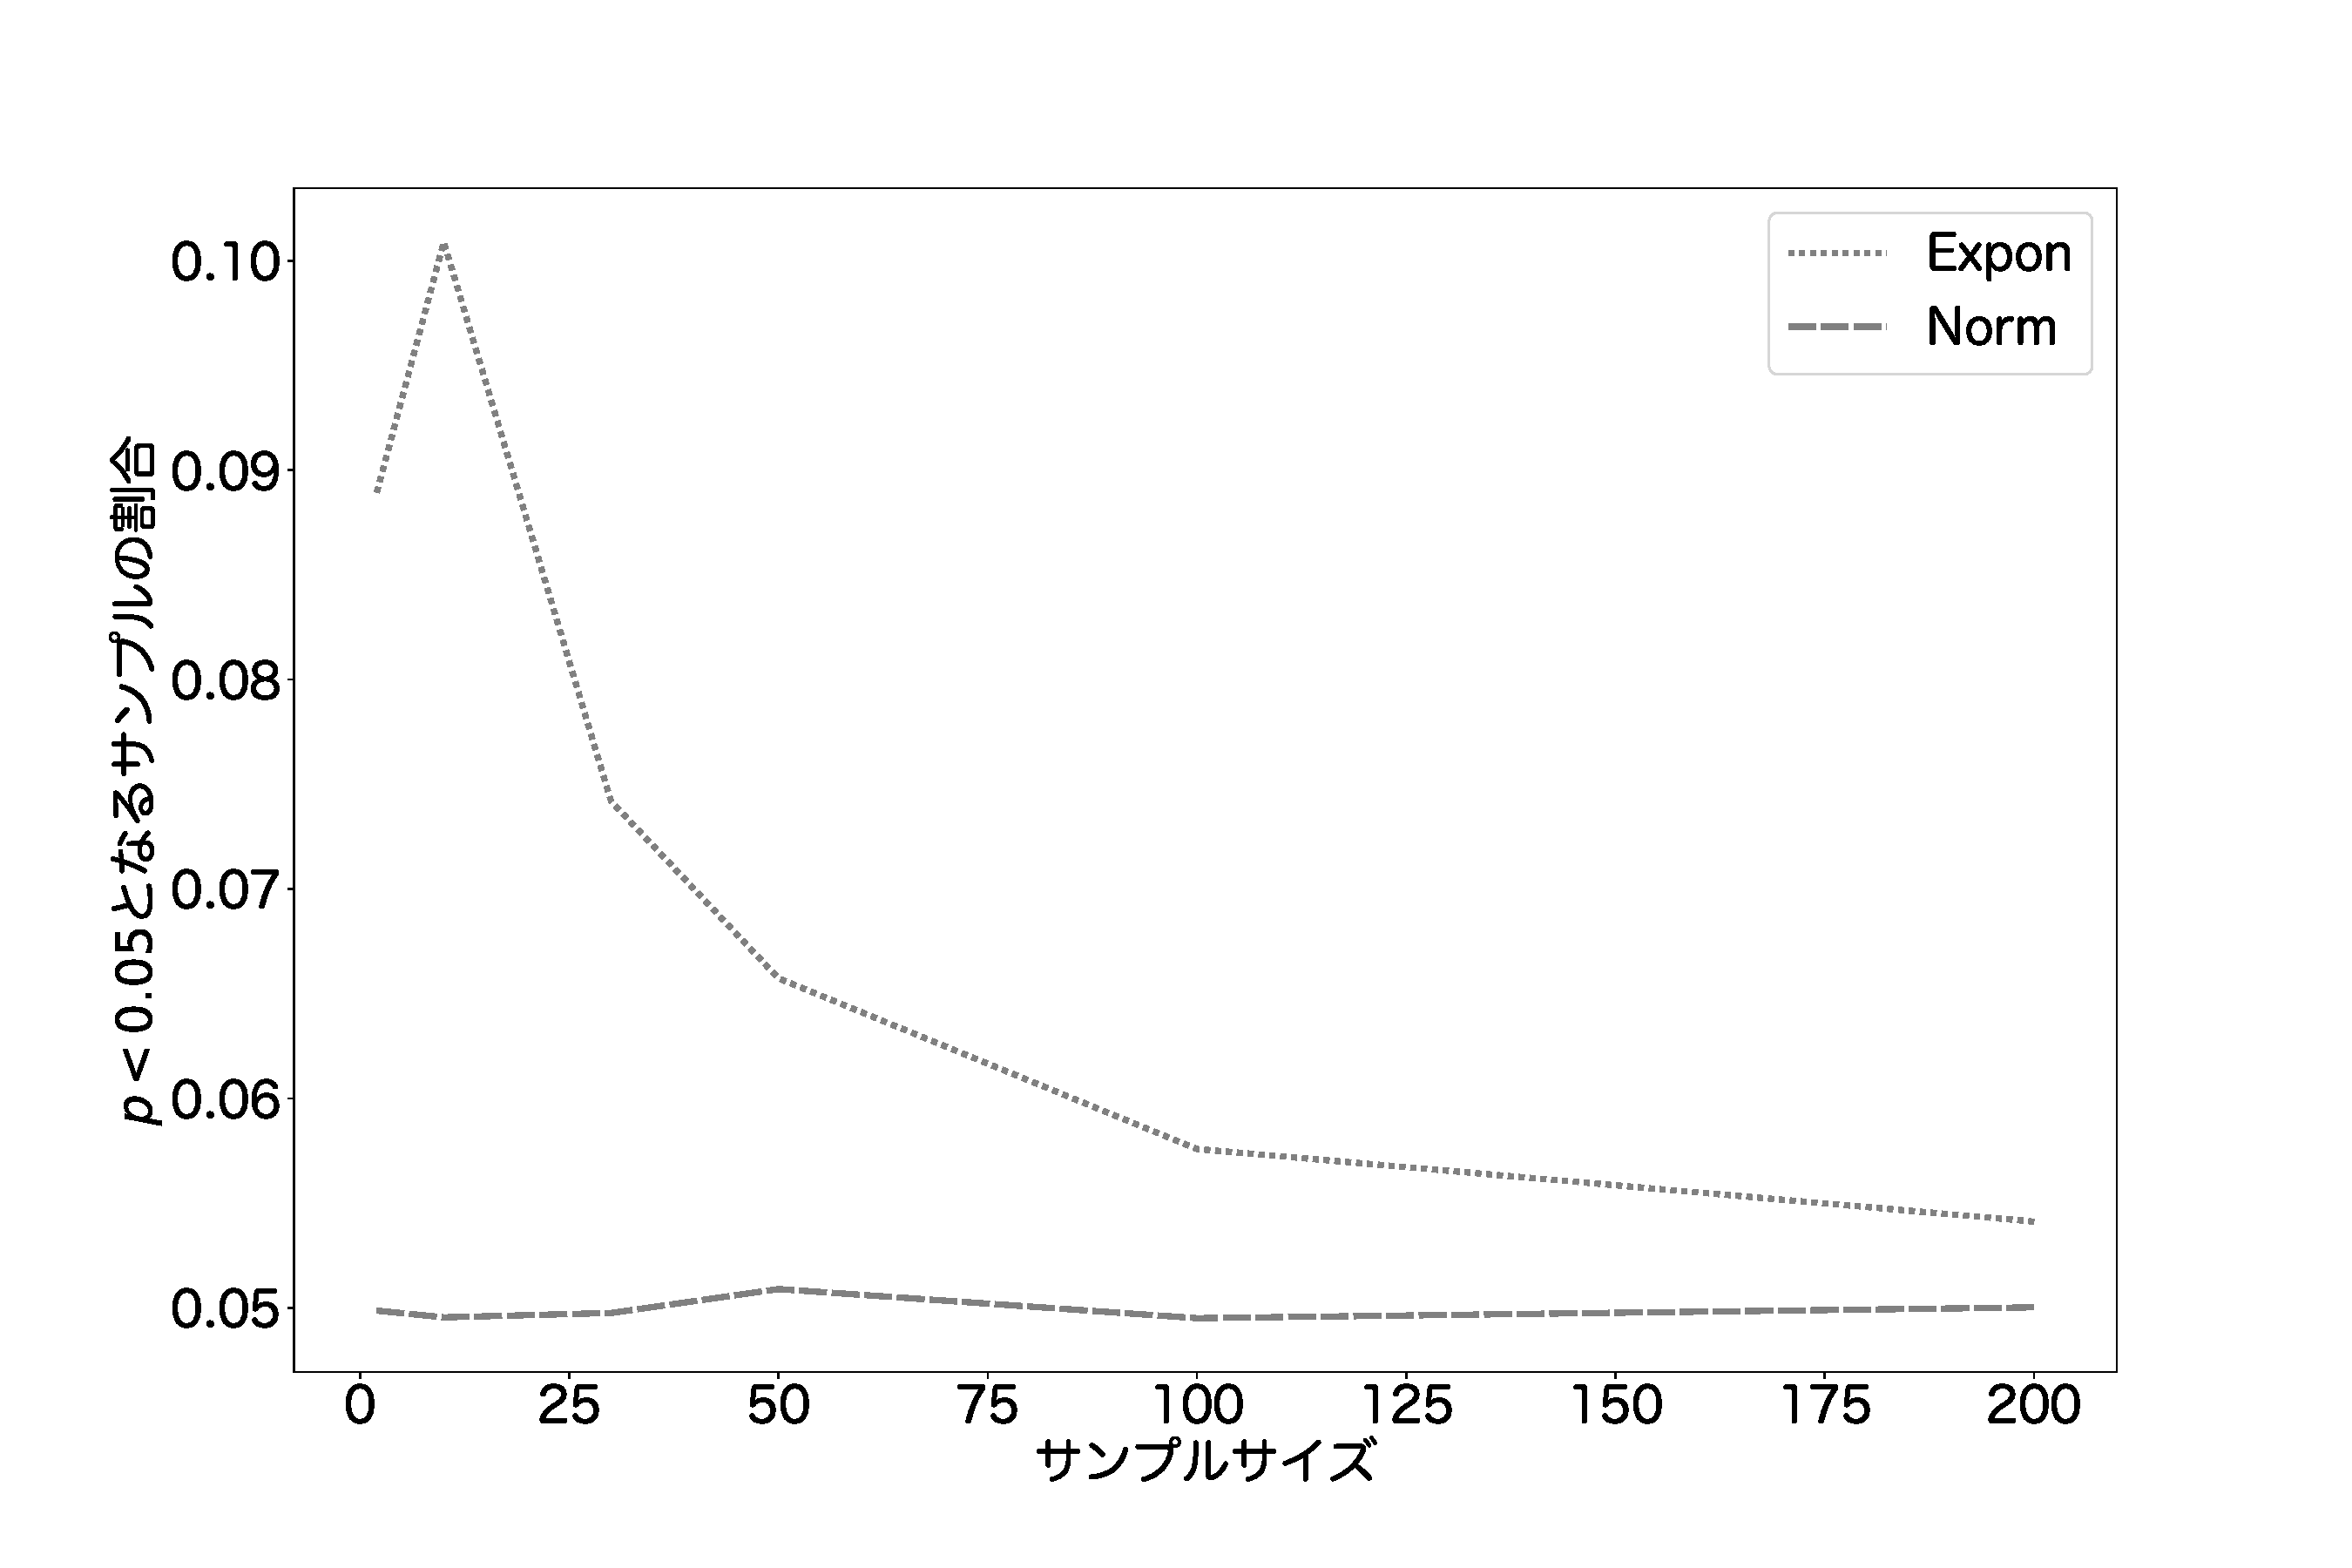
\includegraphics[width=15cm]{./image/04_/t_test_expon_norm.pdf}
        \caption{正規分布または指数ぶんぷから得た標本の$T$値から計算した$p$値で、$p<0.05$以下になる割合}
    \end{center}
\end{figure}

シミュレーションの結果、正規分布から標本を得た場合、$p<0.05$になる割合は、サンプルサイズに依存せず、$5\%$程度であり、理論と一致する。
一方で、指数分布から標本を得た場合、$p<0.05$になる割合はサンプルサイズに応じて変化しており、また、どのサンプルサイズでも$p<0.05$となる割合は$5\%$より多い。
このように、データが正規分布とかけ離れているにもかかわらず、正規分布を含んだ統計モデルを構築し、そこから統計量を計算しても、的外れになることがあることを示唆している\footnote{$n$を大きくしたとき、中心極限定理より、$p<0.05$となる割合も$5\%$に近づくと解釈することがある。本当だろうか。具体的には、次の定理が成り立つのだろうか。
\begin{quote}
\begin{theo}
    $X_1,X_2,\cdots,X_n \sim Exp(\lambda)$とするとき、$T=\frac{\bar{X}-1/\lambda}{\sqrt{\frac{S^2}{n}}}$ここで、$S^2=\frac{1}{n-1}\sum_{i=1}^n(X_i-\bar{X})^2$である。$T\sim t(n-1)$または、$t$がなんらかの統計分布に従う。または、$E[T]<\infty,Var[T]<\infty$
\end{theo}
\end{quote}
このことが成り立つなら、中心極限定理も成立し、$n$が十分大きいときに、分布関数を近似できそうである。
}
\fi
\begin{mybox}
    \begin{quote}
        \paragraph{サンプルサイズがxx以上あるから$t$検定}
        サンプルサイズがある値以上あるので、中心極限定理により、$t$検定が利用できるというものもある\footnote{http://id.ndl.go.jp/bib/024660739}。このロジックが読み込めなかったので、その謎を明らかにすべく我々はアマゾンの奥地へ向かった。

        確かに、サンプルサイズが1以上であれば、$t$検定を行うことは原理的には可能である。
        一方で、データが指数分布的であるときに、$t$検定を使うときに生じる問題は上でみた通りであり、$p<0.05$となる標本の割合が多くなっているので、間違った推測をする可能性が高くなる。
        他の分布関数でもおそらく同じような現象が現れる。
        このことから、我々は「$t$検定が利用可能である」は正確ではなく、「$t$検定を使うことができるが、間違った推測である確率が高くなる」ということだと推察した。
    \end{quote}
\end{mybox}

\subsubsection{検定を繰り返し使おう($\alpha_2$)}
次の統計モデルによって複数の標本について推測することを考える。
\begin{enumerate}
    \item $X_1,X_2,\cdots,X_n $はi.i.d
    \item 正規分布
    \item $\mu$,$\sigma^2=10$
\end{enumerate}
ここまでは、一つの標本に対して、統計モデル$M(\mu)$により推測できるかを考えていた。
ここでは、複数の標本について、$M(\mu)$により推測できるかを仮説検定を指標にし考える。
標本が$3$個あるとする。このとき、それぞれの標本の統計量$T$が信頼区間に入っている確率は、$(1-\alpha)$である。全ての標本の統計量$T$が信頼区間に入っている確率は、その積$(1-\alpha)\times(1-\alpha)\times(1-\alpha)=(1-\alpha)^3$であり、この確率で統計モデルは棄却されない。
一方で、棄却される確率は、$1-(1-\alpha)^3$である。
\begin{table}[hbtp]
    \caption{標本数に応じた$\alpha_2$}
    \label{table:multiple_test_reject_prob}
    \centering
    \begin{tabular}{lcr}
      \hline
      標本数  & $\alpha=0.05$  &  $\alpha=0.01$ \\
      \hline \hline
       1 & $0.05$  & $0.01$ \\
       2 & $0.0975$ & $0.0199$\\
       3 & $0.142$ & $0.0297$\\
       4 & $0.185$ & $0.0394$\\
    \end{tabular}
  \end{table}
表\ref{table:multiple_test_reject_prob}は、標本数に応じた$\alpha_2$である。標本数が大きくなるについれて、$\alpha_2$が大きくなることがわかる。

$\alpha_1$がレベル$\alpha$の検定になっていない場合、$\alpha_2$はさらに有意水準$\alpha$から隔たりの多い数値になる。




\subsection{第二の過誤}
統計モデルの間の類似度を検出力といった。この検出力は、統計モデルに対して、適切な統計量を与えられたときに計算が可能であるが、不適切な統計量を与えたとき、検出力を歪めてしまうことがある。これを第二の過誤(type II error)といい、その確率を$\beta'$で表す。


    
\subsubsection{母集団の標本が指数分布的に分布していた場合}
母集団の分布形と統計モデルに含まれている確率分布関数が著しく異なる場合を考える。
母集団分布の分布として、指数分布を仮定し、そこから無作為抽出によりサンプルサイズ$10^6$の標本を得たとする。
標準偏差の間にサンプルが含まれる確率を計算する。この結果、期待していた値よりも著しく大きな確率$86\%$程度を得る。

\begin{lstlisting}
N = 10**6
sample = expon.rvs(scale=10,size=N)
#sample = norm.rvs(loc=0,scale=1,size=N)
lambd= np.average(sample)
print(np.average(sample),np.std(sample),np.var(sample))

mu = np.average(sample)
s = np.std(sample)

a,b = mu-s,mu+s
len(sample[np.where( (sample >a) & (sample<b) )])/N
\end{lstlisting}

以上でわかるのは、統計モデルと実際の母集団が乖離している場合には、標準誤差に間違いが多くなるということである。
